
%% bare_conf.tex
%% V1.3
%% 2007/01/11
%% by Michael Shell
%% See:
%% http://www.michaelshell.org/
%% for current contact information.
%%
%% This is a skeleton file demonstrating the use of IEEEtran.cls
%% (requires IEEEtran.cls version 1.7 or later) with an IEEE conference paper.
%%
%% Support sites:
%% http://www.michaelshell.org/tex/ieeetran/
%% http://www.ctan.org/tex-archive/macros/latex/contrib/IEEEtran/
%% and
%% http://www.ieee.org/

%%*************************************************************************
%% Legal Notice:
%% This code is offered as-is without any warranty either expressed or
%% implied; without even the implied warranty of MERCHANTABILITY or
%% FITNESS FOR A PARTICULAR PURPOSE!
%% User assumes all risk.
%% In no event shall IEEE or any contributor to this code be liable for
%% any damages or losses, including, but not limited to, incidental,
%% consequential, or any other damages, resulting from the use or misuse
%% of any information contained here.
%%
%% All comments are the opinions of their respective authors and are not
%% necessarily endorsed by the IEEE.
%%
%% This work is distributed under the LaTeX Project Public License (LPPL)
%% ( http://www.latex-project.org/ ) version 1.3, and may be freely used,
%% distributed and modified. A copy of the LPPL, version 1.3, is included
%% in the base LaTeX documentation of all distributions of LaTeX released
%% 2003/12/01 or later.
%% Retain all contribution notices and credits.
%% ** Modified files should be clearly indicated as such, including  **
%% ** renaming them and changing author support contact information. **
%%
%% File list of work: IEEEtran.cls, IEEEtran_HOWTO.pdf, bare_adv.tex,
%%                    bare_conf.tex, bare_jrnl.tex, bare_jrnl_compsoc.tex
%%*************************************************************************

% *** Authors should verify (and, if needed, correct) their LaTeX system  ***
% *** with the testflow diagnostic prior to trusting their LaTeX platform ***
% *** with production work. IEEE's font choices can trigger bugs that do  ***
% *** not appear when using other class files.                            ***
% The testflow support page is at:
% http://www.michaelshell.org/tex/testflow/



% Note that the a4paper option is mainly intended so that authors in
% countries using A4 can easily print to A4 and see how their papers will
% look in print - the typesetting of the document will not typically be
% affected with changes in paper size (but the bottom and side margins will).
% Use the testflow package mentioned above to verify correct handling of
% both paper sizes by the user's LaTeX system.
%
% Also note that the "draftcls" or "draftclsnofoot", not "draft", option
% should be used if it is desired that the figures are to be displayed in
% draft mode.
%
\documentclass[conference]{IEEEtran}

\usepackage{url, fancyvrb, framed, multirow, tabularx, graphicx, epstopdf, enumerate, array, cite, algorithmic, fixltx2e}
\usepackage{float}

\usepackage[cmex10]{amsmath}
\usepackage{algorithm}
\usepackage{listings}
%\usepackage{breqn}

% correct bad hyphenation here
\hyphenation{op-tical net-works semi-conduc-tor}

\begin{document}
%
% paper title
% can use linebreaks \\ within to get better formatting as desired
% \title{A Real-time Gesture Recognition System Using Wireless Signals}
\title{Several Applications of Wireless Signals Using Channel State Information (CSI)}

% author names and affiliations
% use a multiple column layout for up to three different
% affiliations
%\author{\IEEEauthorblockN{Michael Shell}
%\IEEEauthorblockA{School of Electrical and\\Computer Engineering\\
%Georgia Institute of Technology\\
%Atlanta, Georgia 30332--0250\\
%Email: http://www.michaelshell.org/contact.html}
%\and
%\IEEEauthorblockN{Homer Simpson}
%\IEEEauthorblockA{Twentieth Century Fox\\
%Springfield, USA\\
%Email: homer@thesimpsons.com}
%\and
%\IEEEauthorblockN{James Kirk\\ and Montgomery Scott}
%\IEEEauthorblockA{Starfleet Academy\\
%San Francisco, California 96678-2391\\
%Telephone: (800) 555--1212\\
%Fax: (888) 555--1212}}

% conference papers do not typically use \thanks and this command
% is locked out in conference mode. If really needed, such as for
% the acknowledgment of grants, issue a \IEEEoverridecommandlockouts
% after \documentclass

% for over three affiliations, or if they all won't fit within the width
% of the page, use this alternative format:
%
%\author{\IEEEauthorblockN{Michael Shell\IEEEauthorrefmark{1},
%Homer Simpson\IEEEauthorrefmark{2},
%James Kirk\IEEEauthorrefmark{3},
%Montgomery Scott\IEEEauthorrefmark{3} and
%Eldon Tyrell\IEEEauthorrefmark{4}}
%\IEEEauthorblockA{\IEEEauthorrefmark{1}School of Electrical and Computer Engineering\\
%Georgia Institute of Technology,
%Atlanta, Georgia 30332--0250\\ Email: see http://www.michaelshell.org/contact.html}
%\IEEEauthorblockA{\IEEEauthorrefmark{2}Twentieth Century Fox, Springfield, USA\\
%Email: homer@thesimpsons.com}
%\IEEEauthorblockA{\IEEEauthorrefmark{3}Starfleet Academy, San Francisco, California 96678-2391\\
%Telephone: (800) 555--1212, Fax: (888) 555--1212}
%\IEEEauthorblockA{\IEEEauthorrefmark{4}Tyrell Inc., 123 Replicant Street, Los Angeles, California 90210--4321}}
\author{
\IEEEauthorblockN{Yuning Mao}
\IEEEauthorblockA{
IEEE Honored Class\\
Shanghai Jiao Tong University\\
morningmoni@sjtu.edu.cn}
\and
\IEEEauthorblockN{Yuting Jia}
\IEEEauthorblockA{
IEEE Honored Class\\
Shanghai Jiao Tong University\\
XXX@sjtu.edu.cn}
\and
\IEEEauthorblockN{Zhenfeng Shi}
\IEEEauthorblockA{
IEEE Honored Class\\
Shanghai Jiao Tong University\\
XXX@sjtu.edu.cn}
}

% use for special paper notices
%\IEEEspecialpapernotice{(Invited Paper)}


% make the title area
\maketitle


\begin{abstract}
Wireless signals (e.g., WiFi) are almost everywhere nowadays. However, the research of wireless signals using channel state information (CSI) has just started. In this project, we try several applications by leveraging the channel state information (CSI). We implement an end-to-end system which can be used to control electronic devices (e.g., laptop) by gesture recognition. We also do experiments of indoor localization using CSI.  Our system leverages the WiFi signals using off-the-shelf network interface card (Intel 5300). It achieves an average accuracy of XXX \% for a classification of 4? typical gestures and XXX\% for localization of 5 different tables in the lab.

\end{abstract}
% IEEEtran.cls defaults to using nonbold math in the Abstract.
% This preserves the distinction between vectors and scalars. However,
% if the conference you are submitting to favors bold math in the abstract,
% then you can use LaTeX's standard command \boldmath at the very start
% of the abstract to achieve this. Many IEEE journals/conferences frown on
% math in the abstract anyway.

% no keywords

\begin{keywords}
Channel State Information(CSI), Gesture Recognition, Indoor Localization, Wireless Signals, Signal Processing, Classification
\end{keywords}


% For peer review papers, you can put extra information on the cover
% page as needed:
% \ifCLASSOPTIONpeerreview
% \begin{center} \bfseries EDICS Category: 3-BBND \end{center}
% \fi
%
% For peerreview papers, this IEEEtran command inserts a page break and
% creates the second title. It will be ignored for other modes.
\IEEEpeerreviewmaketitle

\section{Introduction}
As the users shift from traditional PCs to mobile devices and their expectation for new methods of interaction increases, there are increasing demands for novel human-computer interfaces (HCI) through which the users can control various applications.
Among those recently proposed methods, gesture recognition has gained much popularity. There are now successful commercial devices such as XBOX Kinect and Leap Motion. 
However, the cost of these commercial devices is relatively high and it also takes efforts to install and set up them.
In addition, these devices only support in-sight gesture recognition since they are vision-based.
Researchers also developed ways to move the sensors onto the body so as to bolster out-of-sight scenarios, and yet wearing sensors itself is inconvenient and infeasible in many cases.

Nowadays, wireless signals are almost everywhere. They are used for communication, remote control and so on. However, the research of doing gesture recognition by leveraging wireless signals just started in 2013. It partially results from the fact that there are plenty of challenges when it comes to the use of wireless signals. 
Wireless signals are usually unstable and sensitive to environmental changes, there could be issues because of medium contention, multipath interference, noises caused by other objects and so on.
collecting wireless signals and processing them is hence challenging.
Recently proposed WiFi-based systems are based on analyzing the changes caused by human motion in the characteristics of the wireless signals, such as the received signal strength indicator (RSSI) or detailed channel state information (CSI).
We consider this a new direction of research and hence did some experiments by leveraging the CSI.
The CSI is helpful for many purposes, such as gesture recognition, indoor localization, keystroke recognition, human activity detection and so on.
In this paper, we propose an end-to-end gesture recognition system and implement a demo using off-the-shelf network interface card (Intel 5300) and \emph{CSI Tools} \cite{halperin2011tool}. 

Different from previous methods, we use machine learning techniques to support classification of different gestures and the accuracy of the classification can hence increase as the users provide more samples.
We also support user-defined gestures. All the users need is to perform a gesture several times and then the system can store the pattern and recognize the gesture afterwards.
In addition, We did experiment of indoor localization, or rather, classifying five tables in the lab.
The results show that...

The rest of this paper is organized as follows.  The background is introduced in Section \ref{section-background}. The system design is illustrated in Section \ref{section-design}. Section \ref{section-evaluation} demonstrates the evaluation of the system by multiple experiments. The discussion concerning limitations, division of work, and future work is presented in Section \ref{section-discussion}. Section \ref{section-conclusion} concludes the paper.

\section{Background} \label{section-background}

\subsection{Channel State Information (CSI)}
Modern WiFi devices that support IEEE 802.11n/ac standard typically consist of multiple transmit and multiple receive antennas and thus support MIMO. Each MIMO channel between each transmit-receive (TX-RX) antenna pair of a transmitter and receiver comprises of multiple subcarriers. These WiFi devices continuously monitor the state of the wireless channel to effectively perform transmit power allocations and rate adaptations for each individual MIMO stream such that the available capacity of the wireless channel is maximally utilized \cite{halperin2010802}. These devices quantify the state of the channel in terms of CSI values. The CSI values essentially characterize the Channel Frequency Response (CFR) for each subcarrier between each transmit-receive (TX-RX) antenna pair.
Let $M_T$ denote the number of transmit antennas, $M_R$ denote the number of receive antennas and $S_c$ denote the number of OFDM subcarriers. Let $X_i$ and $Y_i$ represent the $M_T$ dimensional transmitted signal vector and $M_R$ dimensional received signal vector, respectively, for subcarrier i and let Ni represent an $M_R$ dimensional noise vector. An $M_R \times M_T$ MIMO system at any time instant can be represented by the following equation.
\begin{equation}
	Y_i = H_iX_i + N_i, i \in [1, S_c]
\end{equation}
In the equation above, the $M_R \times M_T$ dimensional channel matrix $H_i$ represents the Channel State Information (CSI) for the subcarrier $i$. Any two communicating WiFi devices estimate this channel matrix $H_i$ for every subcarrier by regularly transmitting a known preamble of OFDM symbols between each other \cite{ali2015keystroke}. For each Tx-Rx antenna pair, we can attain CSI values for $S_c$ = 30 OFDM subcarriers of the 20 MHz WiFi Channel by using CSI Tools and Intel 5300 network interface card. This leads to 30 matrices with dimensions $M_R \times M_T$ per CSI sample.
\subsection{Related Work}
There are a myriad of work for device-free gesture recognition. Some are based on Received Signal Strength Indicator (RSSI), some on the detailed Channel State Information (CSI).

\cite{pu2013whole} claims itself to be the first to do gesture recognition using wireless signals. 
They presented a system named WiSee, which extracts minute Doppler shifts from wide-band OFDM transmissions to enable whole-home sensing and recognition of human gestures.
There is another work \emph{Allsee} \cite{kellogg2014bringing} which leverages wireless signals furthermore and applies the method into RFID tags and power-harvesting sensors.  AllSee consumes three to four orders of magnitude lower power than state-of-the-art systems and can enable always-on gesture recognition for smartphones and tablet.

Another category is RSSI-based gesture recognition, which leverages the signal strength changes caused by human motion.
However, due to the low resolution of RSSI values provided by commercial devices, the performance of these kinds of methods is usually considered relatively low.
For instance, the accuracy is 56\% over 7 different gestures in \cite{sigg2014telepathic}.
Nevertheless, \cite{abdelnasser2015wigest} claims that they achieve 96\% when evaluating the system using a multi-media player application.
they also claim that they only need standard WiFi device, unlike \emph{Wisee} which uses USRP in their experiment.

There are also other applications based on CSI. \cite{wang2015understanding} \cite{wang2014eyes} \cite{wang2015robust} use it to do human activity recognition. They examine channel features and can uniquely identify both in-place activities and walking movements across a home by comparing them
against signal profiles.
\cite{ali2015keystroke} uses it to recognize keystroke. The idea is similar: while typing a certain key, the hands and fingers of a user move in a unique formation and direction and thus generate a unique pattern in the time-series of CSI values.
Some even use CSI to do voice recognition. \cite{wang2014we} presented WiHear, which enables WiFi signals to ``hear'' people's talks without deploying any devices.
Another direction is to use CSI to do indoor localization. The CSI can be used as fingerprints of various locations. Recent work can be found at \cite{hosen2015utilizing} \cite{kotaru2015spotfi} \cite{li2015passive} \cite{yang2015enhancing} \cite{jiang2014communicating} \cite{chen2014fine}.
\section{System Design} \label{section-design}
\subsection{Overview}
In this section, we describe the whole process and flow of work. It consists of data collection, data processing and model training. For data collection, we introduce the hardware and software tools and our work above them. For data processing, we discuss signal filtering methods we implemented. For model training, we illustrate how we select the features and model.
\subsection{Data Collection}

CSI Tool \cite{halperin2011tool} is a toolkit released in 2011 and it is open-source on github. However, the tool relies on the authors' custom firmware image which only works on the Intel 5300 NIC.
We hence installed an Intel 5300 network card into a Lenovo R400 laptop as the receive side of wireless signals and followed the instruction on the official website to install the CSI Tool.
\begin{figure}[H]
\begin{center}
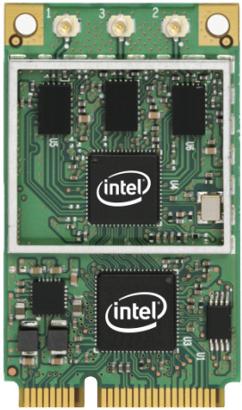
\includegraphics[width=1in]{NIC.png}
\caption{Intel 5300 network interface card}
\end{center}
\end{figure}
We measure the CSI of received packets using the CSI Tool at a sampling rate of 1000 HZ. For each segment of data, the CSI is represented in 30 channels, as a figure below:
\begin{figure}[H]
\begin{center}
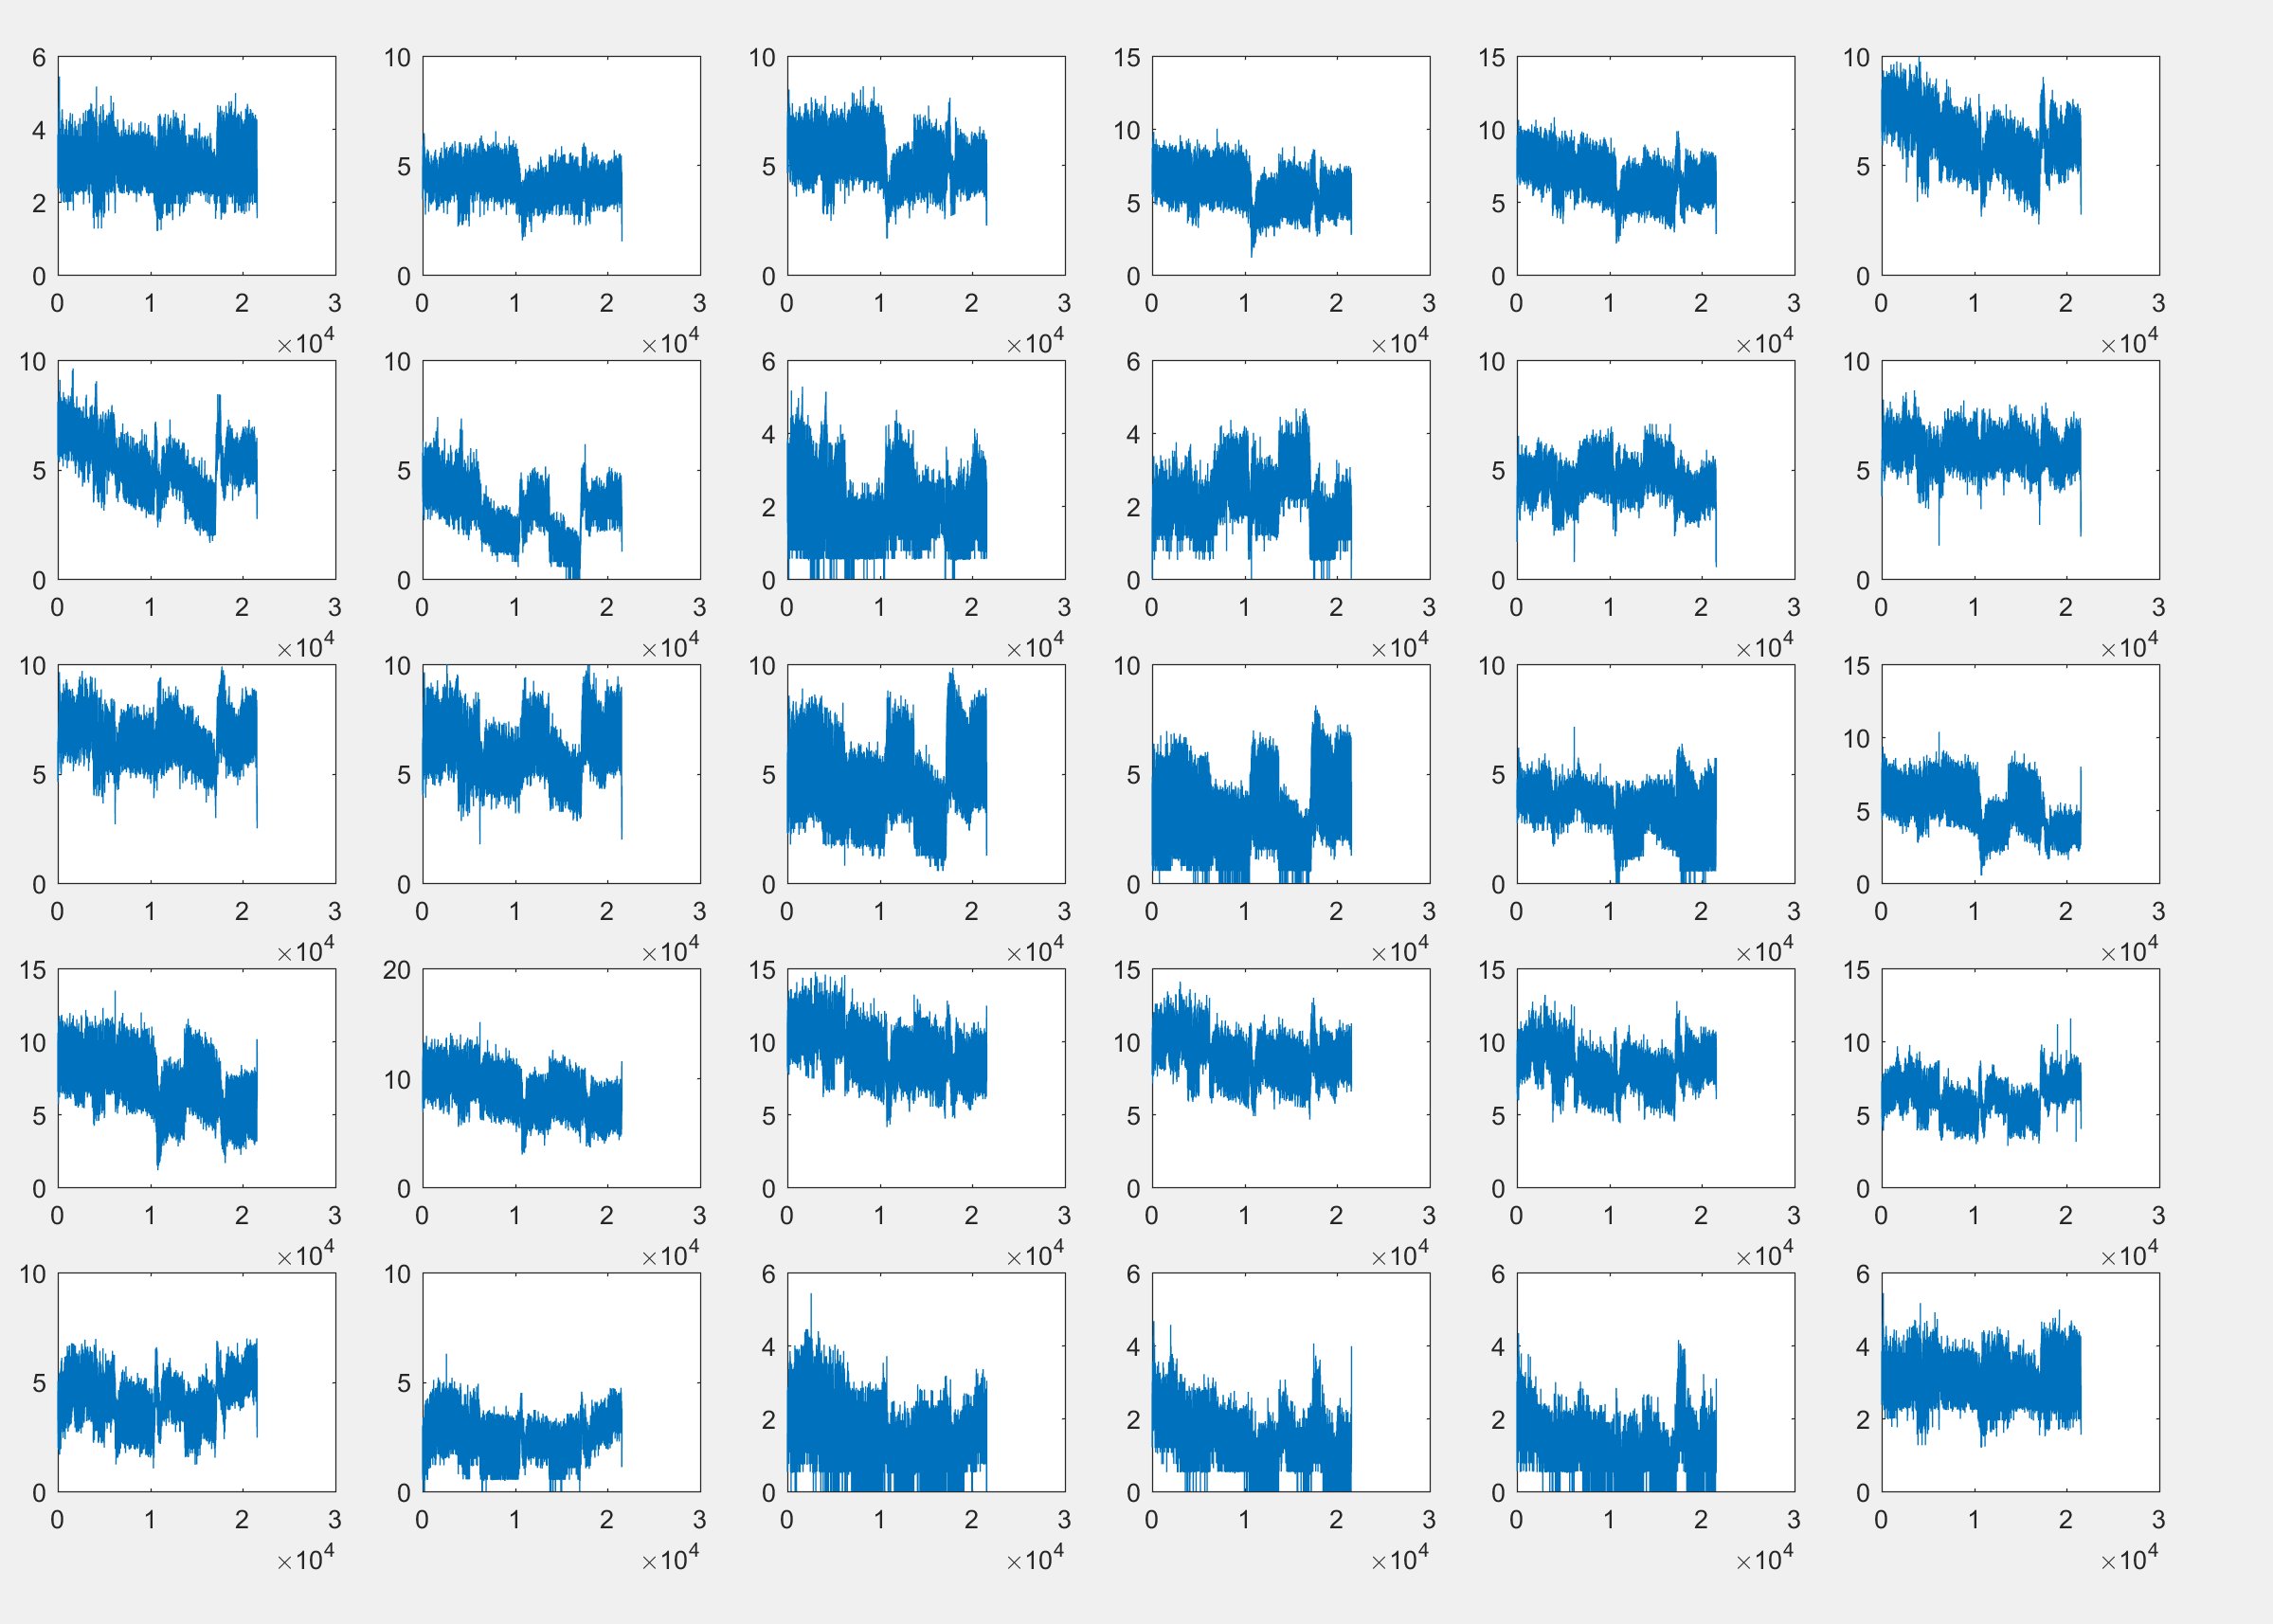
\includegraphics[width=3in]{Original.png}
\caption{Raw signal in 30 channel of CSI}
\end{center}
\end{figure}
From the above figure, we can see that the trend of the signal is obscure. Therefore, we need to preprocess the signals to attain signals with high SNR before we can do feature selection and model training.

The data format we can acquire is as follows \cite{halperin2011tool}:
\begin{enumerate}
\item \textbf{timestamp\_low} is the low 32 bits of the NIC's 1 MHz clock. It wraps about every 4300 seconds, or 72 minutes. This field was not yet recorded in the sample trace, so all values are arbitrary and always equal 4.

\item \textbf{bfee\_count} is simply a count of the total number of beamforming measurements that have been recorded by the driver and sent to userspace. The netlink channel between the kernel and userspace is lossy, so these can be used to detect measurements that were dropped in this pipe.

\item \textbf{Nrx} represents the number of antennas used to receive the packet by this NIC, and Ntx represents the number of space/time streams transmitted. In this case, the sender sent a single-stream packet and the receiver used all 3 antennas to receive it.

\item \textbf{rssi\_a, rssi\_b, and rssi\_c} correspond to RSSI measured by the receiving NIC at the input to each antenna port. This measurement is made during the packet preamble. This value is in dB relative to an internal reference; to get the received signal strength in dBm we must combine it with the Automatic Gain Control (AGC) setting (agc) in dB and also subtract off a magic constant. This process is explained below.

\item \textbf{perm} tells us how the NIC permuted the signals from the 3 receive antennas into the 3 RF chains that process the measurements. The sample value of [3 2 1] implies that Antenna C was sent to RF Chain A, Antenna B to Chain B, and Antenna A to Chain C. This operation is performed by an antenna selection module in the NIC and generally corresponds to ordering the antennas in decreasing order of RSSI.

\item \textbf{rate} is the rate at which the packet was sent, in the same format as the rate\_n\_flags defined above. Note that the antenna bits are omitted, as there is no way for the receiver to know which transmit antennas were used.

\item \textbf{csi} is the CSI itself, normalized to an internal reference. It is a $N_{tx} \times N_{rx} \times 30$ 3-D matrix where the third dimension is across 30 subcarriers in the OFDM channel. For a 20 MHz-wide channel, these correspond to about half the OFDM subcarriers, and for a 40 MHz-wide channel, this is about one in every 4 subcarriers. Which subcarriers were measured is defined by the IEEE 802.11n-2009 standard.
\end{enumerate}

The CSI Tool provides supplementary programs written in Matlab to preprocess the signals.

It uses the following command to store the CSI into a binary file.
{ 
\scriptsize
\begin{lstlisting}[language=SH]
sudo linux-80211n-csitool-supplementary/netlink/log_to_file csi.dat
\end{lstlisting}
}

Then it uses Matlab to read the binary file and does the preprocessing.
{ 
\scriptsize
\begin{lstlisting}[language=MATLAB]
csi_trace = read_bf_file('sample_data/log.all_csi.6.7.6');
plot(db(abs(squeeze(csi).')))
legend('RX Antenna A', 'RX Antenna B', 'RX Antenna C', 
	'Location', 'SouthEast' );
xlabel('Subcarrier index');
ylabel('SNR [dB]');
\end{lstlisting}
}

Which can display the SNR of three different antennas on subcarrier level.
\begin{figure}[H]
\centering
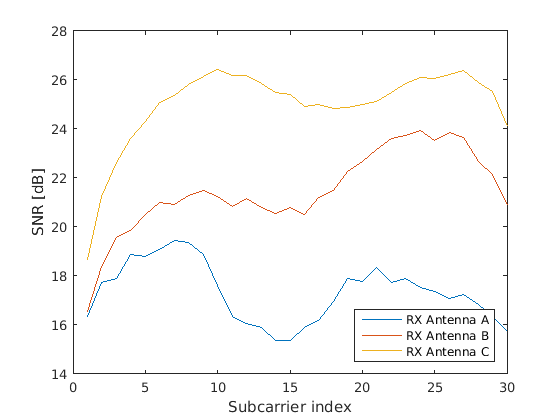
\includegraphics[width=3in]{SNR.png}
\caption{The SNR of three antennas}
\end{figure}

To adjust the process above to our own purpose, we modified \textbf{log\_to\_file.c} to allow it to stop logging at certain time. We also used C to rewrite the functions in \textbf{read\_bf\_file.m} which were originally written in Matlab. MORE DETAIL HERE @JYT.


\subsection{Data Processing}
We use the amplitude of CSI from 30 subcarriers as the raw input.
Then we do low-pass filtering and moving average filtering in turn.
\subsubsection{Low-pass Filtering}
Our raw data is sampled at a sampling rate of 1000 HZ, which is relatively high since the duration of typical human gestures is greater than hundreds of milliseconds. Therefore, we run CSI in the wireless signals through a low-pass filter to smooth out the fast varying noise while keeping the variations caused by gestures intact.

In our design, we use a low-pass filter with the following parameters:
\begin{table}[H]
\centering
\begin{tabular}{|c|c|}
\hline
Parameter & value \\
\hline
\hline
Sampling Frequency & 1000 Hz \\
\hline
Passband Frequency & 80 Hz \\
\hline
Stopband Frequency & 100 Hz \\
\hline
Passband Ripple & 1 dB \\
\hline
Stopband Attenuation & 60 dB \\
\hline
\end{tabular}
\caption{Parameters for low-pass filter}
\end{table}

The frequency response is shown as follows:
\begin{figure}[H]
\centering
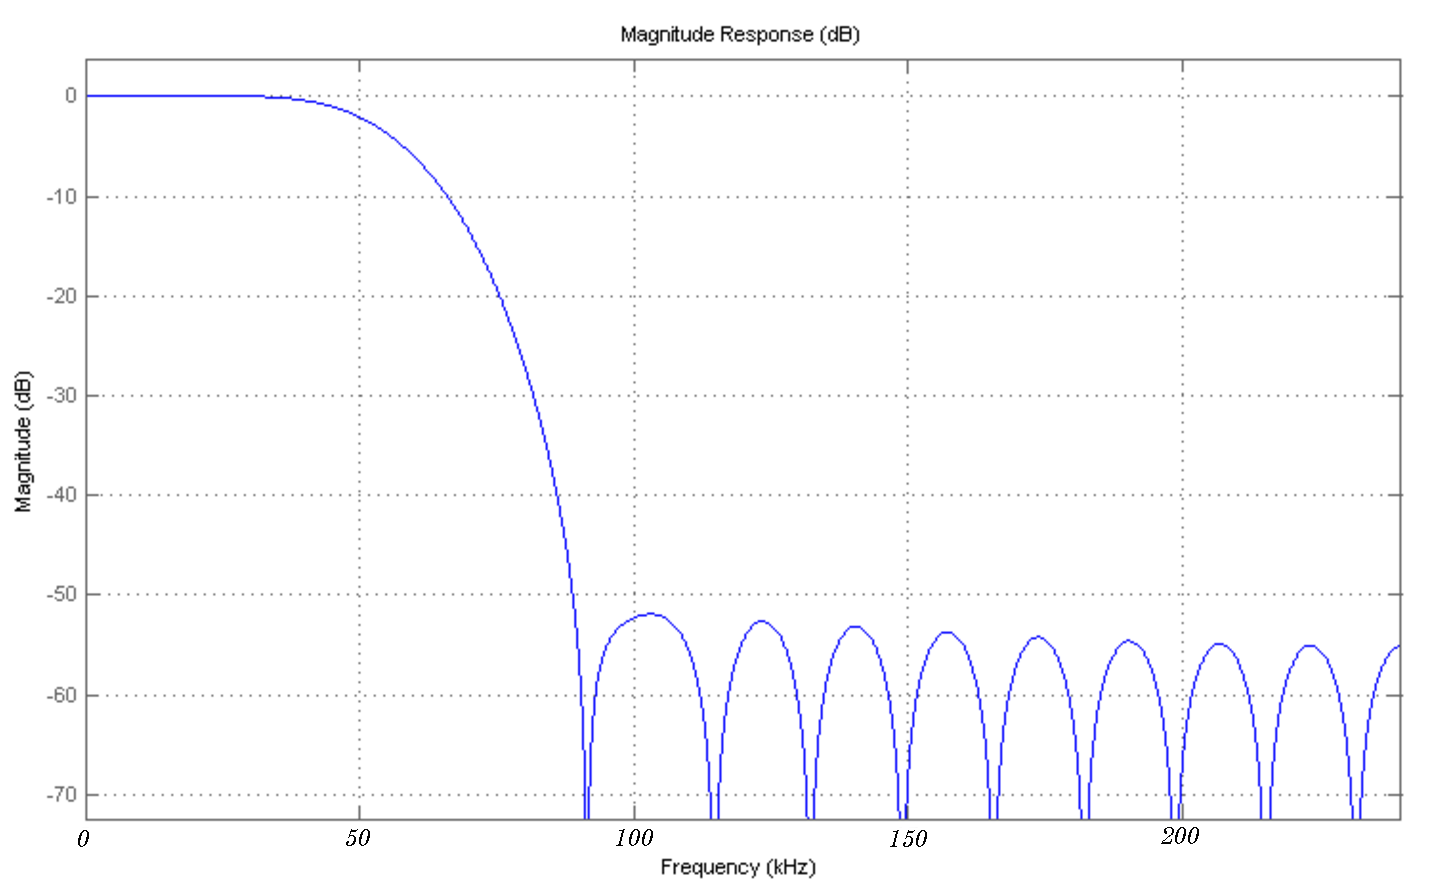
\includegraphics[width=3in]{FR.png}
\caption{Frequency Response}
\end{figure}
The result of passing raw signals to this filter is as follows:
\begin{figure}[H]
\centering
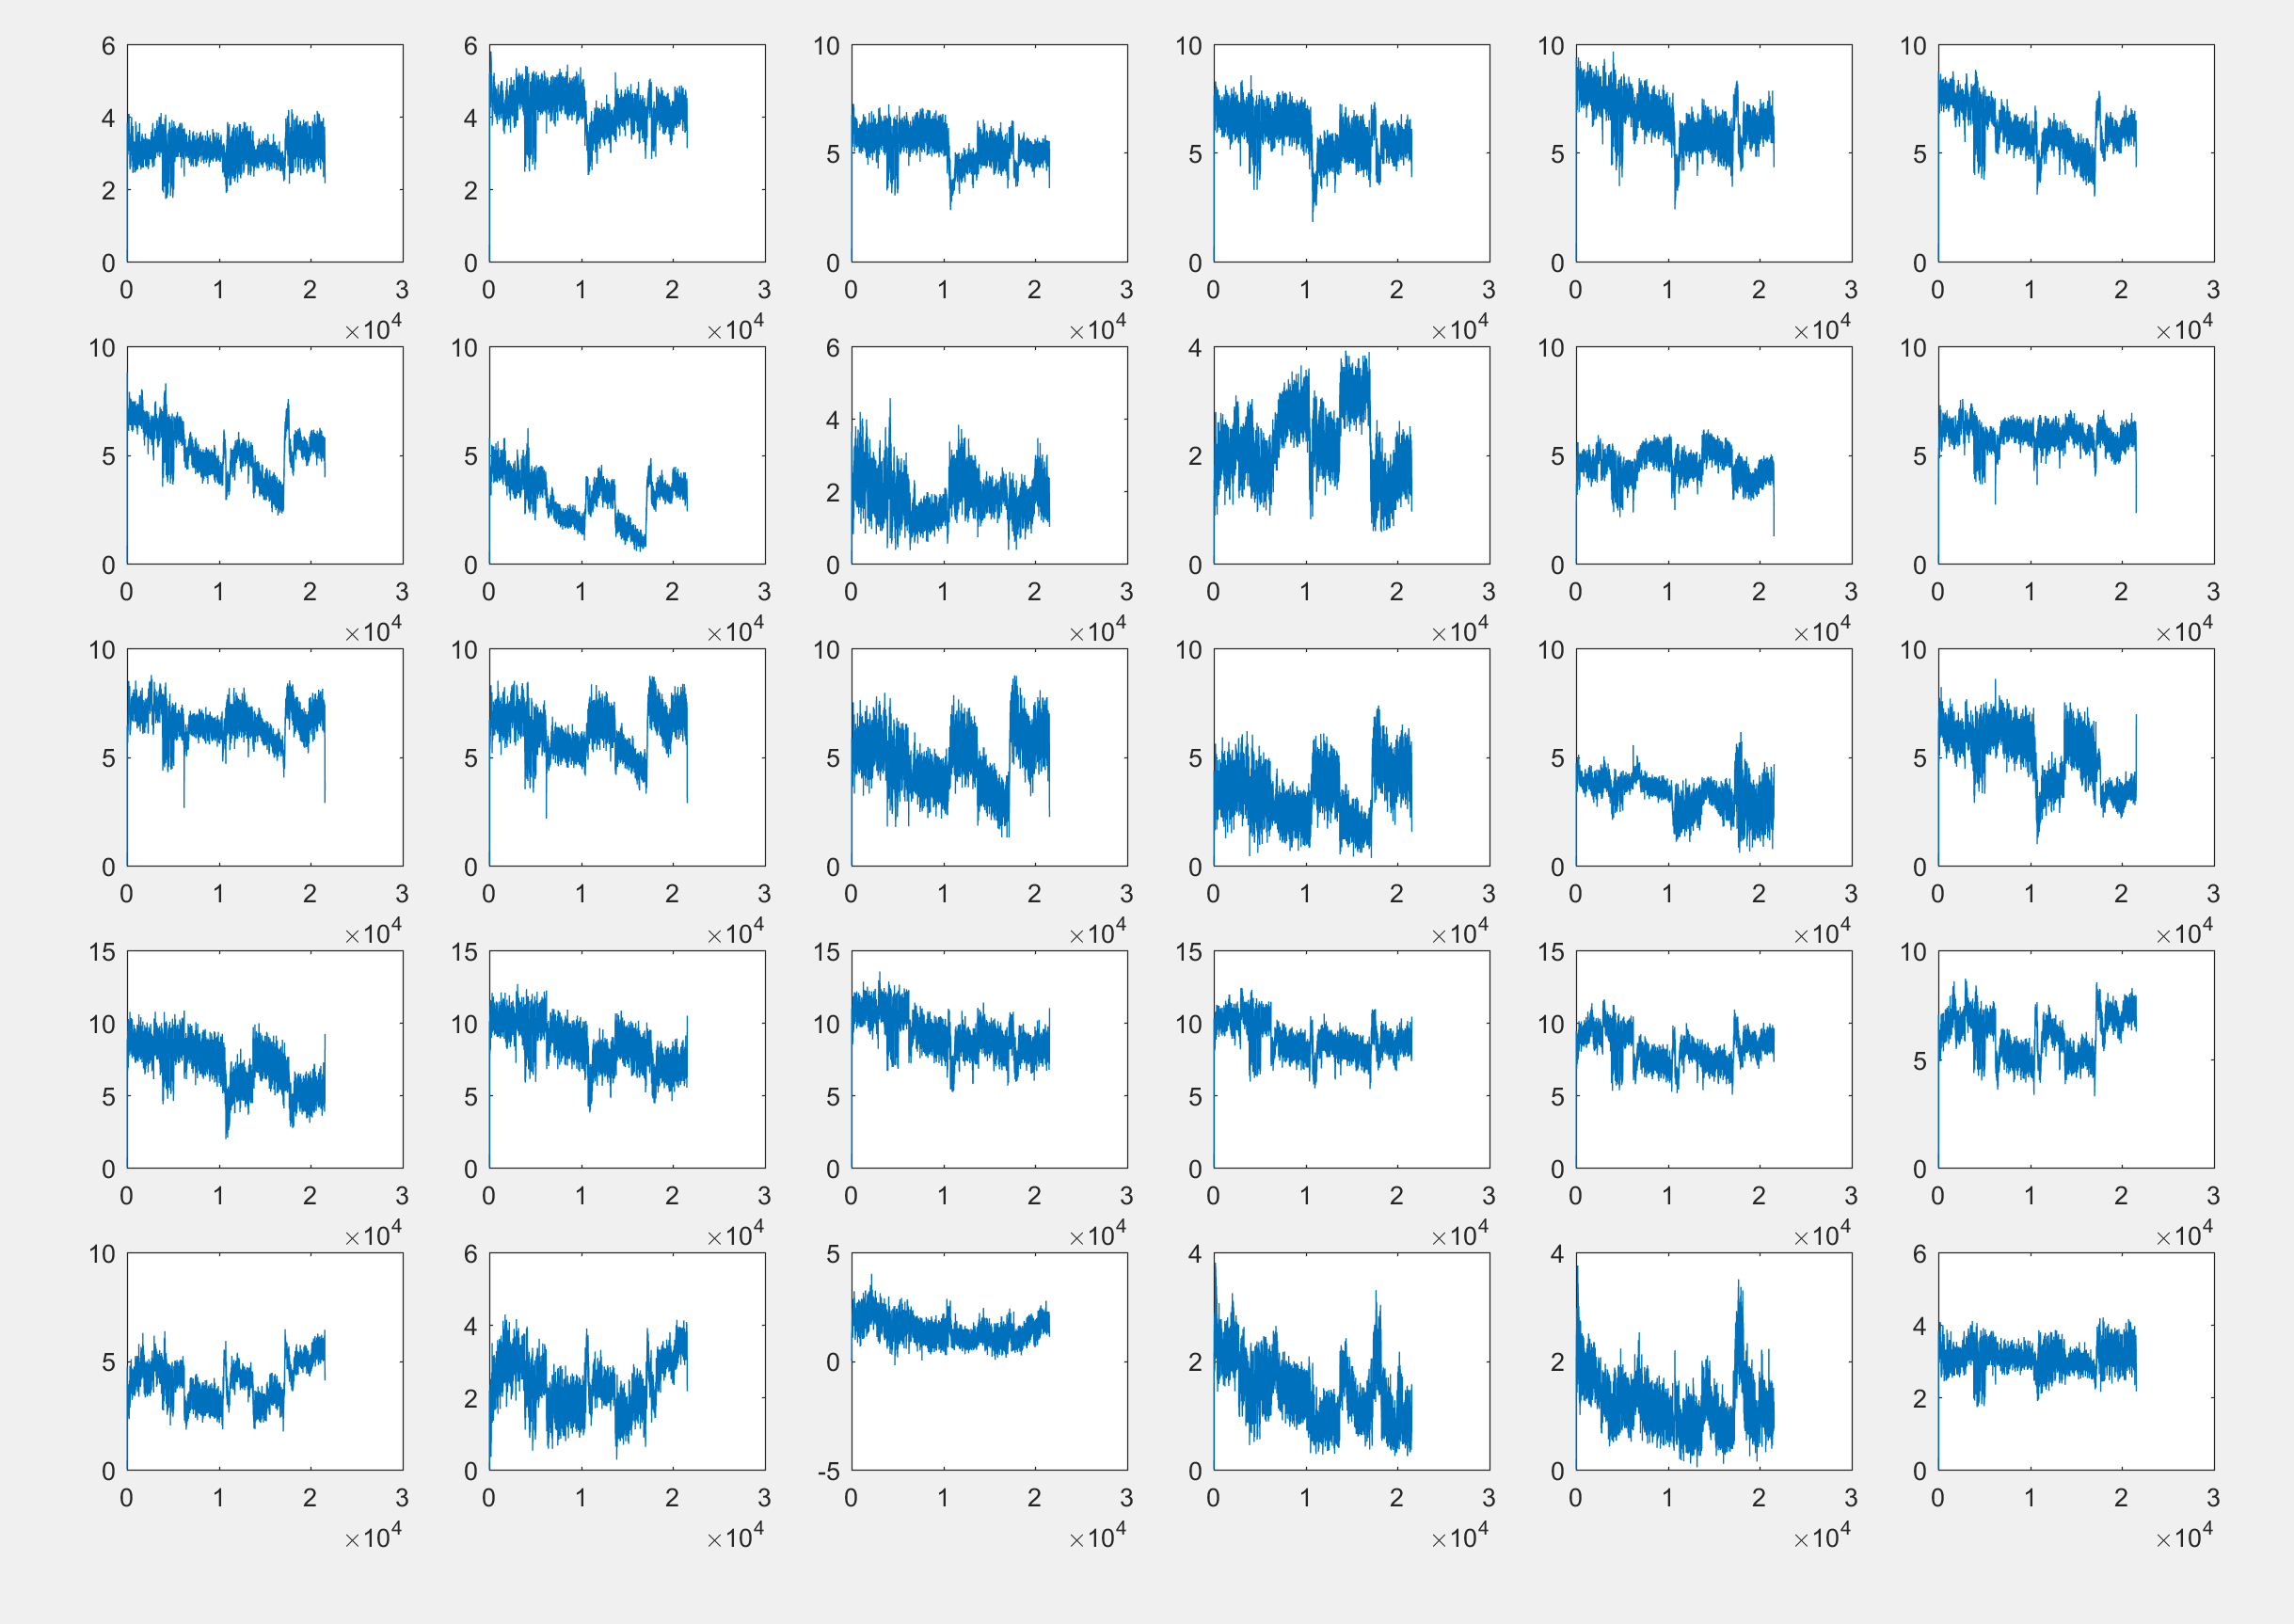
\includegraphics[width=3in]{LPF.png}
\caption{Result of low-pass filter}
\end{figure}

Notably, we have implemented such low-pass filter both in Matlab and Python to meet our requirement.
In Matlab, we directly use a build-in Butterworth filter but adjust the parameters to the needed ones.
\begin{algorithm}
	\centering
	\caption{Low-pass filter implement in MATLAB}
	\begin{algorithmic}
	\STATE function y=LowPassFilter(x) 
	\STATE \qquad h = fdesign.lowpass(Fpass, Fstop, Apass, Astop, Fs) 
	\STATE \qquad Hd = butter(h, 'MatchExactly', match) 
	\STATE \qquad y = filter(Hd, x) 
	\STATE end
	\end{algorithmic}
\end{algorithm}
Matlab provides a more powerful and convenient method based on \emph{fdesign} to design filters, compared to the traditional way like \emph{fdatool}. As is illustrated above, only 3 lines of code can accomplish filter implementation.

However, Matlab is slow to start and run. And since the model we use is written in Python, we turn to the implementation of python version. In Python, the implementation of such a low-pass filter is slightly harder than it in Matlab. We use an open-source package for mathematics, science and engineering called \emph{Scipy}. In this package, it includes a toolbox called \emph{Scipy.signal} which contains some filtering functions, a limited set of filter design tools and a few B-spline interpolation algorithms for one- and two-dimensional data.

In detail, the filter is implemented as a direct II transposed structure as follows:
$$a[0]*y[n] = b[0]*x[n] + b[1]*x[n-1] + ... + b[nb]*x[n-nb]$$
                        $$- a[1]*y[n-1] - ... - a[na]*y[n-na]$$
using the following difference equations:
\begin{algorithm}[H]
y[m] = b[0]*x[m] + z[0,m-1] \\
z[0,m] = b[1]*x[m] + z[1,m-1] - a[1]*y[m]\\
...\\
z[n-3,m] = b[n-2]*x[m] + z[n-2,m-1] - a[n-2]*y[m]\\
z[n-2,m] = b[n-1]*x[m] - a[n-1]*y[m]\\
\end{algorithm}
where m is the output sample number and $n=max(len(a), len(b))$ is the model order.

The rational transformation function describing this filter in the z-transform domain is:
$$Y(z) = \frac{b[0]b[1]z^{-1}+...+b[nb]z^{-nb}}{a[0]+a[1]z^{-1}+...+a[na]z^{-na}}X(z)$$

The pseudocode is as follows:
\begin{algorithm}
\centering
	\caption{Low-pass filter implement in Python}
	\begin{algorithmic}
	\STATE def LowPass(cutoff, fs, order=5) 
	\STATE \qquad nyq = $0.5$ * fs
	\STATE \qquad normal\_cutoff = cutoff / nyq
	\STATE \qquad b, a = butter(order, normal\_cutoff, 
	\STATE \qquad \qquad \qquad \qquad btype='low', analog=False)
	\STATE \qquad return b, a

	\STATE def LowPassFilter(x, cutoff, fs, order=5) 
	\STATE \qquad b, a = LowPass(cutoff, fs, order=order)
	\STATE \qquad y = lfilter(b, a, x)
	\STATE \qquad return y
	\end{algorithmic}
\end{algorithm}

\subsubsection{Moving Average Filtering}
Another serious problem is that minor changes in various environmental factors such as user location, distance between router and receiver, and objects in vicinity, can have an impact on the absolute WiFi channel amplitude. The amplitude changes we are interested in for gesture recognition, however, are independent of these absolute values. To extract these changes and remove bias from the absolute values, we filter the samples by calculating a windowed average of the channel samples (averaged over 300 ms, which is 300 points based on our sampling rate) from the low-pass filtered samples in the previous step.

The following figure shows the result of the moving average filter.
\begin{figure}[H]
\centering
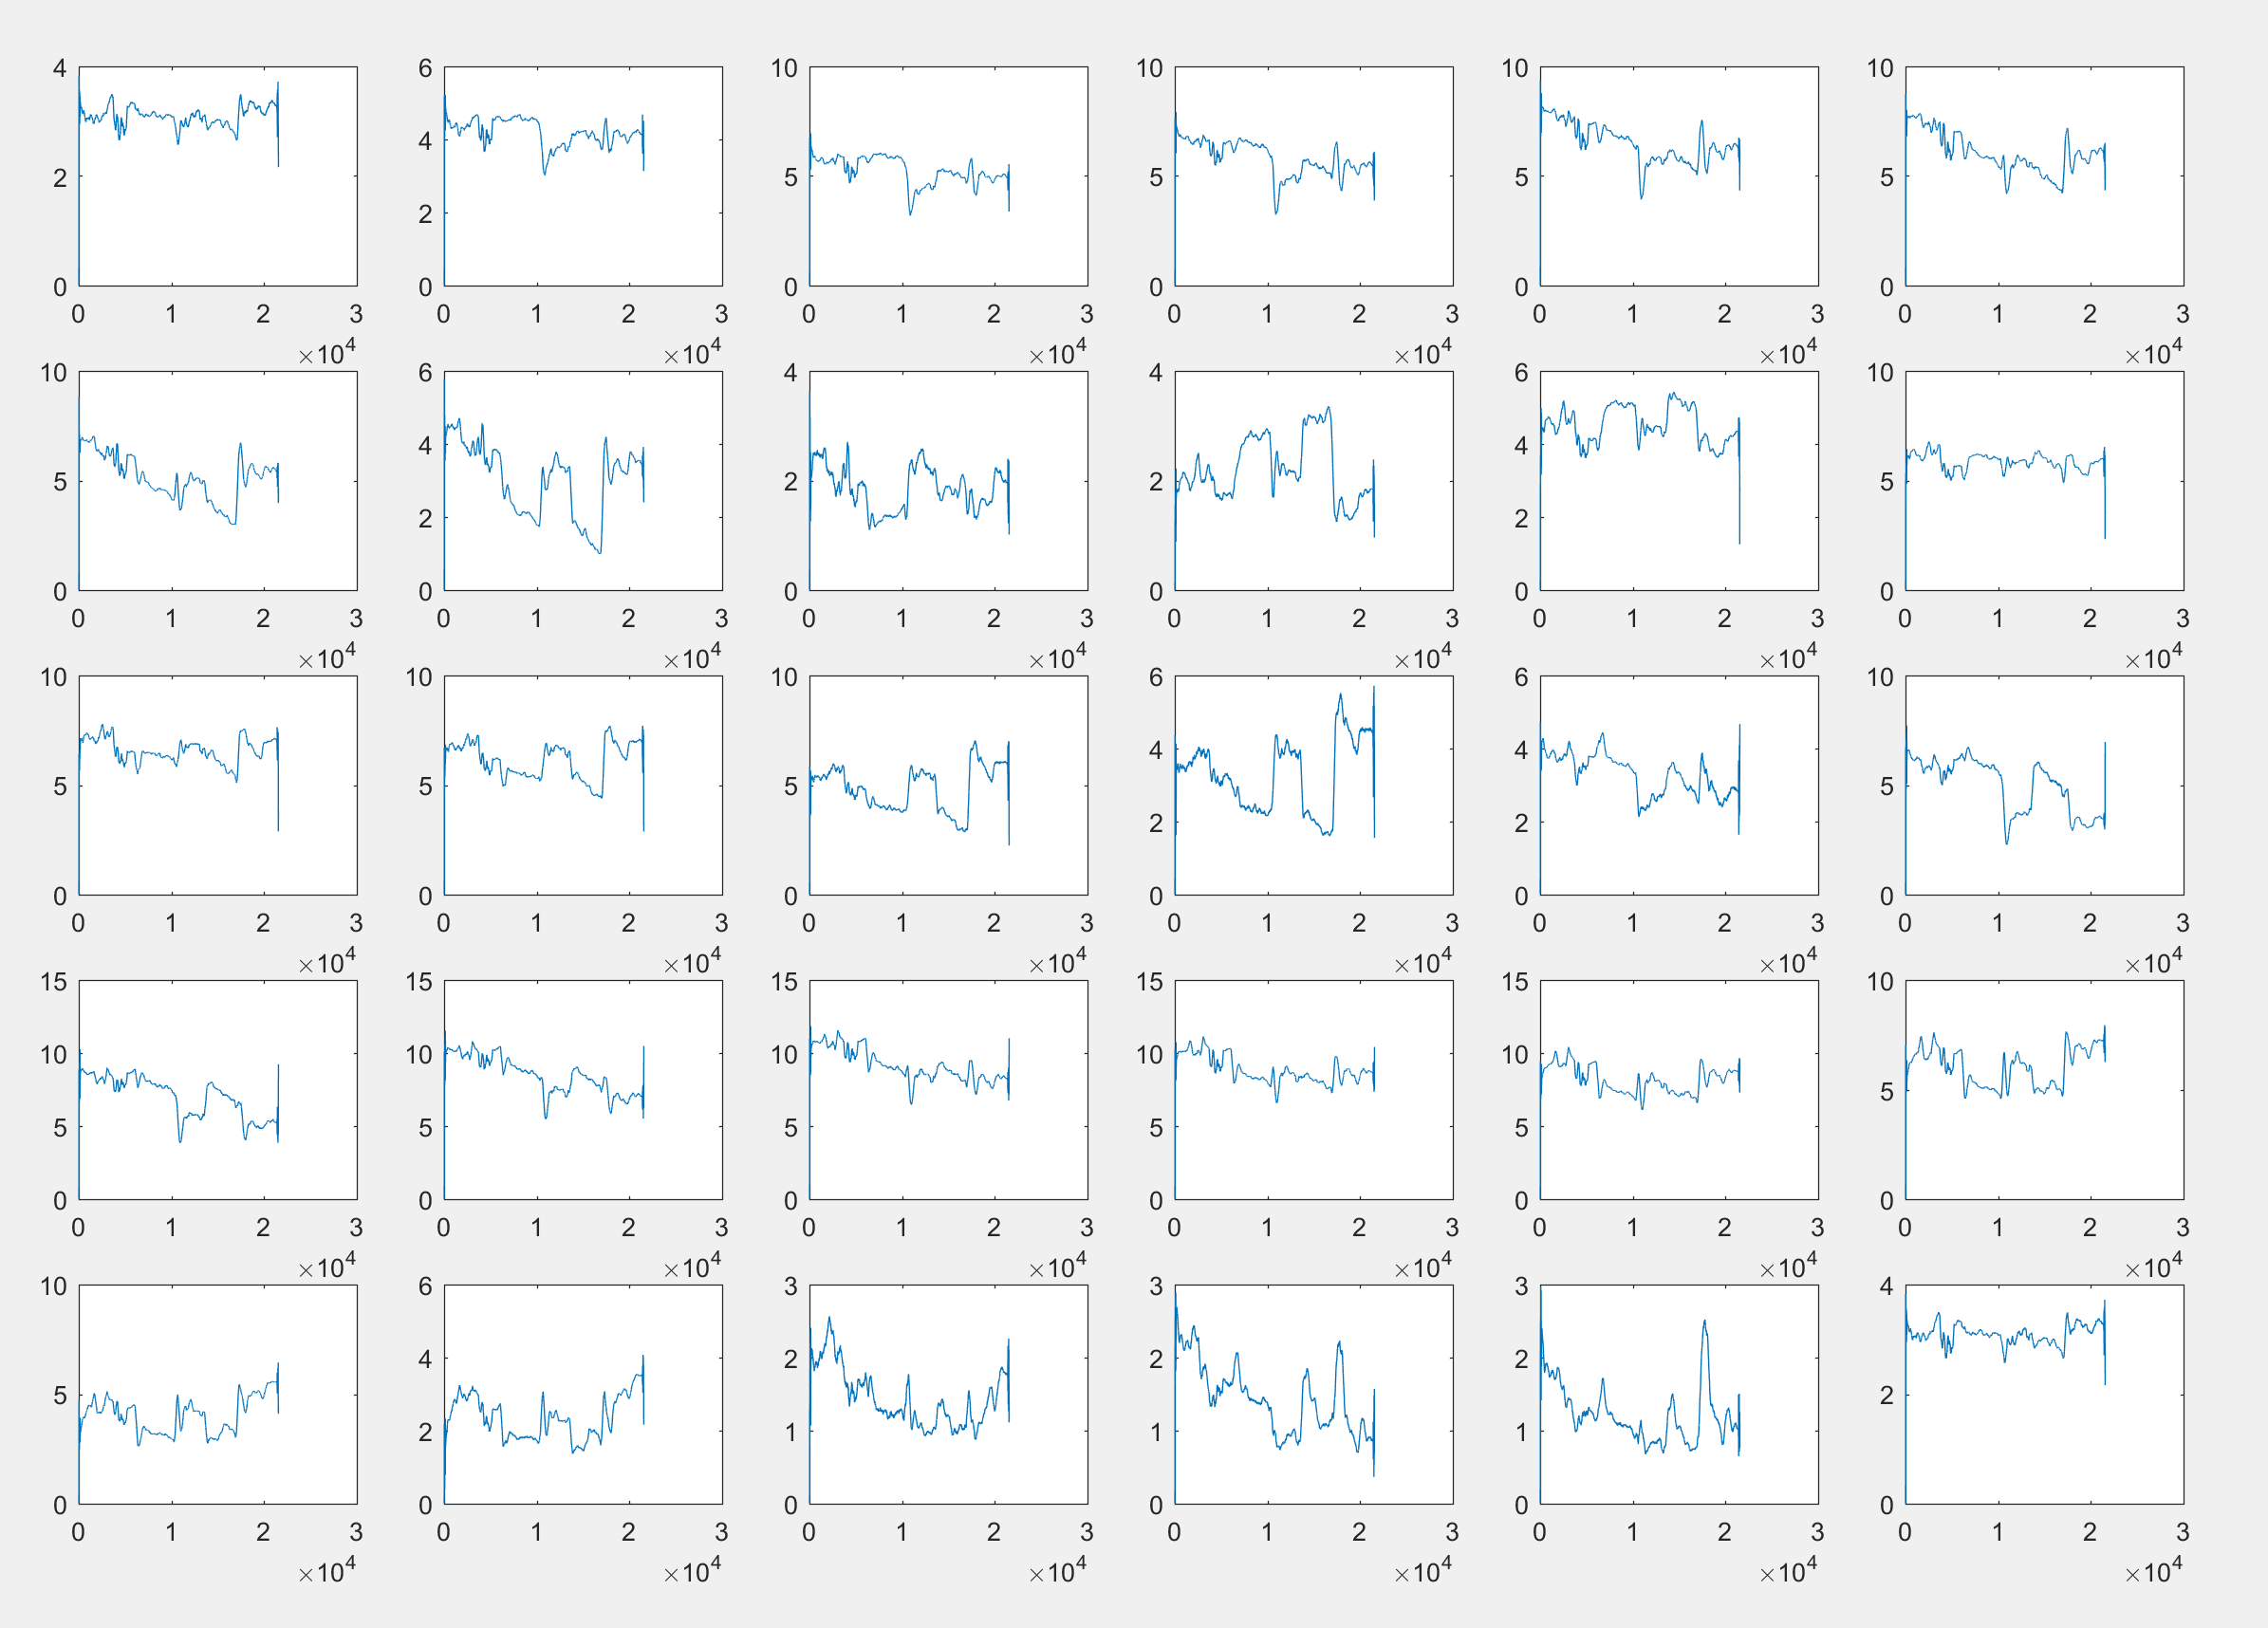
\includegraphics[width=3in]{MAF.png}
\caption{Result of moving-average filter}
\end{figure}
From the above figure, we can clearly see the trend of the signal comparing to the raw data.

Similar to the low-pass filter, we also implement two moving average filter on Matlab and Python.

In MATLAB, we use a build-in filter which filters the input data, x, using a rational transformation function defined by the numerator and denominator coefficients b and a, respectively.

Here we design
\begin{algorithm}[H]
b=ones(1, moving\_points)/moving\_points\\
a=1
\end{algorithm}
In this case, the filter is identical to a moving average implementation.

The pseudocode is as follows:
\begin{algorithm}
\centering
	\caption{Moving average filter implement in MATLAB}
	\begin{algorithmic}
	\STATE function y=MovingSmoothing(x) 
	\STATE \qquad moving\_points = 301;
	\STATE \qquad y = filter(ones(1, moving\_point)/moving\_point, 1, x);
	\STATE end
	\end{algorithmic}
\end{algorithm}

In Python, no such build-in function can be call to fulfill the filtering. Therefore, we implement it by ourselves, which has a complexity of $O(n)$.

The pseudocode is as follows:
\begin{algorithm}
\centering
	\caption{Moving average filter implement in Python}
	\begin{algorithmic}
	\STATE def MeanMovingSmoothing(x, windowSize):
    \STATE \qquad y = np.zeros(x.size)
    \STATE \qquad for i in range(0, windowSize // 2):
    \STATE \qquad \qquad y[i] = x[i]
    \STATE \qquad for i in range((x.size - windowSize // 2), x.size):
    \STATE \qquad \qquad y[i] = x[i]
    \STATE \qquad summation = x[:windowSize].sum()
    \STATE \qquad y[windowSize // 2] = summation / windowSize
    \STATE \qquad for i in range(windowSize // 2 + 1
    \STATE \qquad \qquad \qquad \qquad , x.size - windowSize // 2):
    \STATE \qquad \qquad summation = summation - 
    \STATE \qquad \qquad \qquad \qquad x[i - windowSize // 2 - 1] 
    \STATE \qquad \qquad \qquad \qquad + x[i + windowSize // 2]
    \STATE \qquad \qquad y[i] = summation / windowSize
    \STATE \qquad return y
	\end{algorithmic}
\end{algorithm}
\subsubsection{Some Example Result of Preprocessing}
In this section, we illustrate some figures of the result of preprocessing procedure described as above.
\begin{figure}[H]
\centering
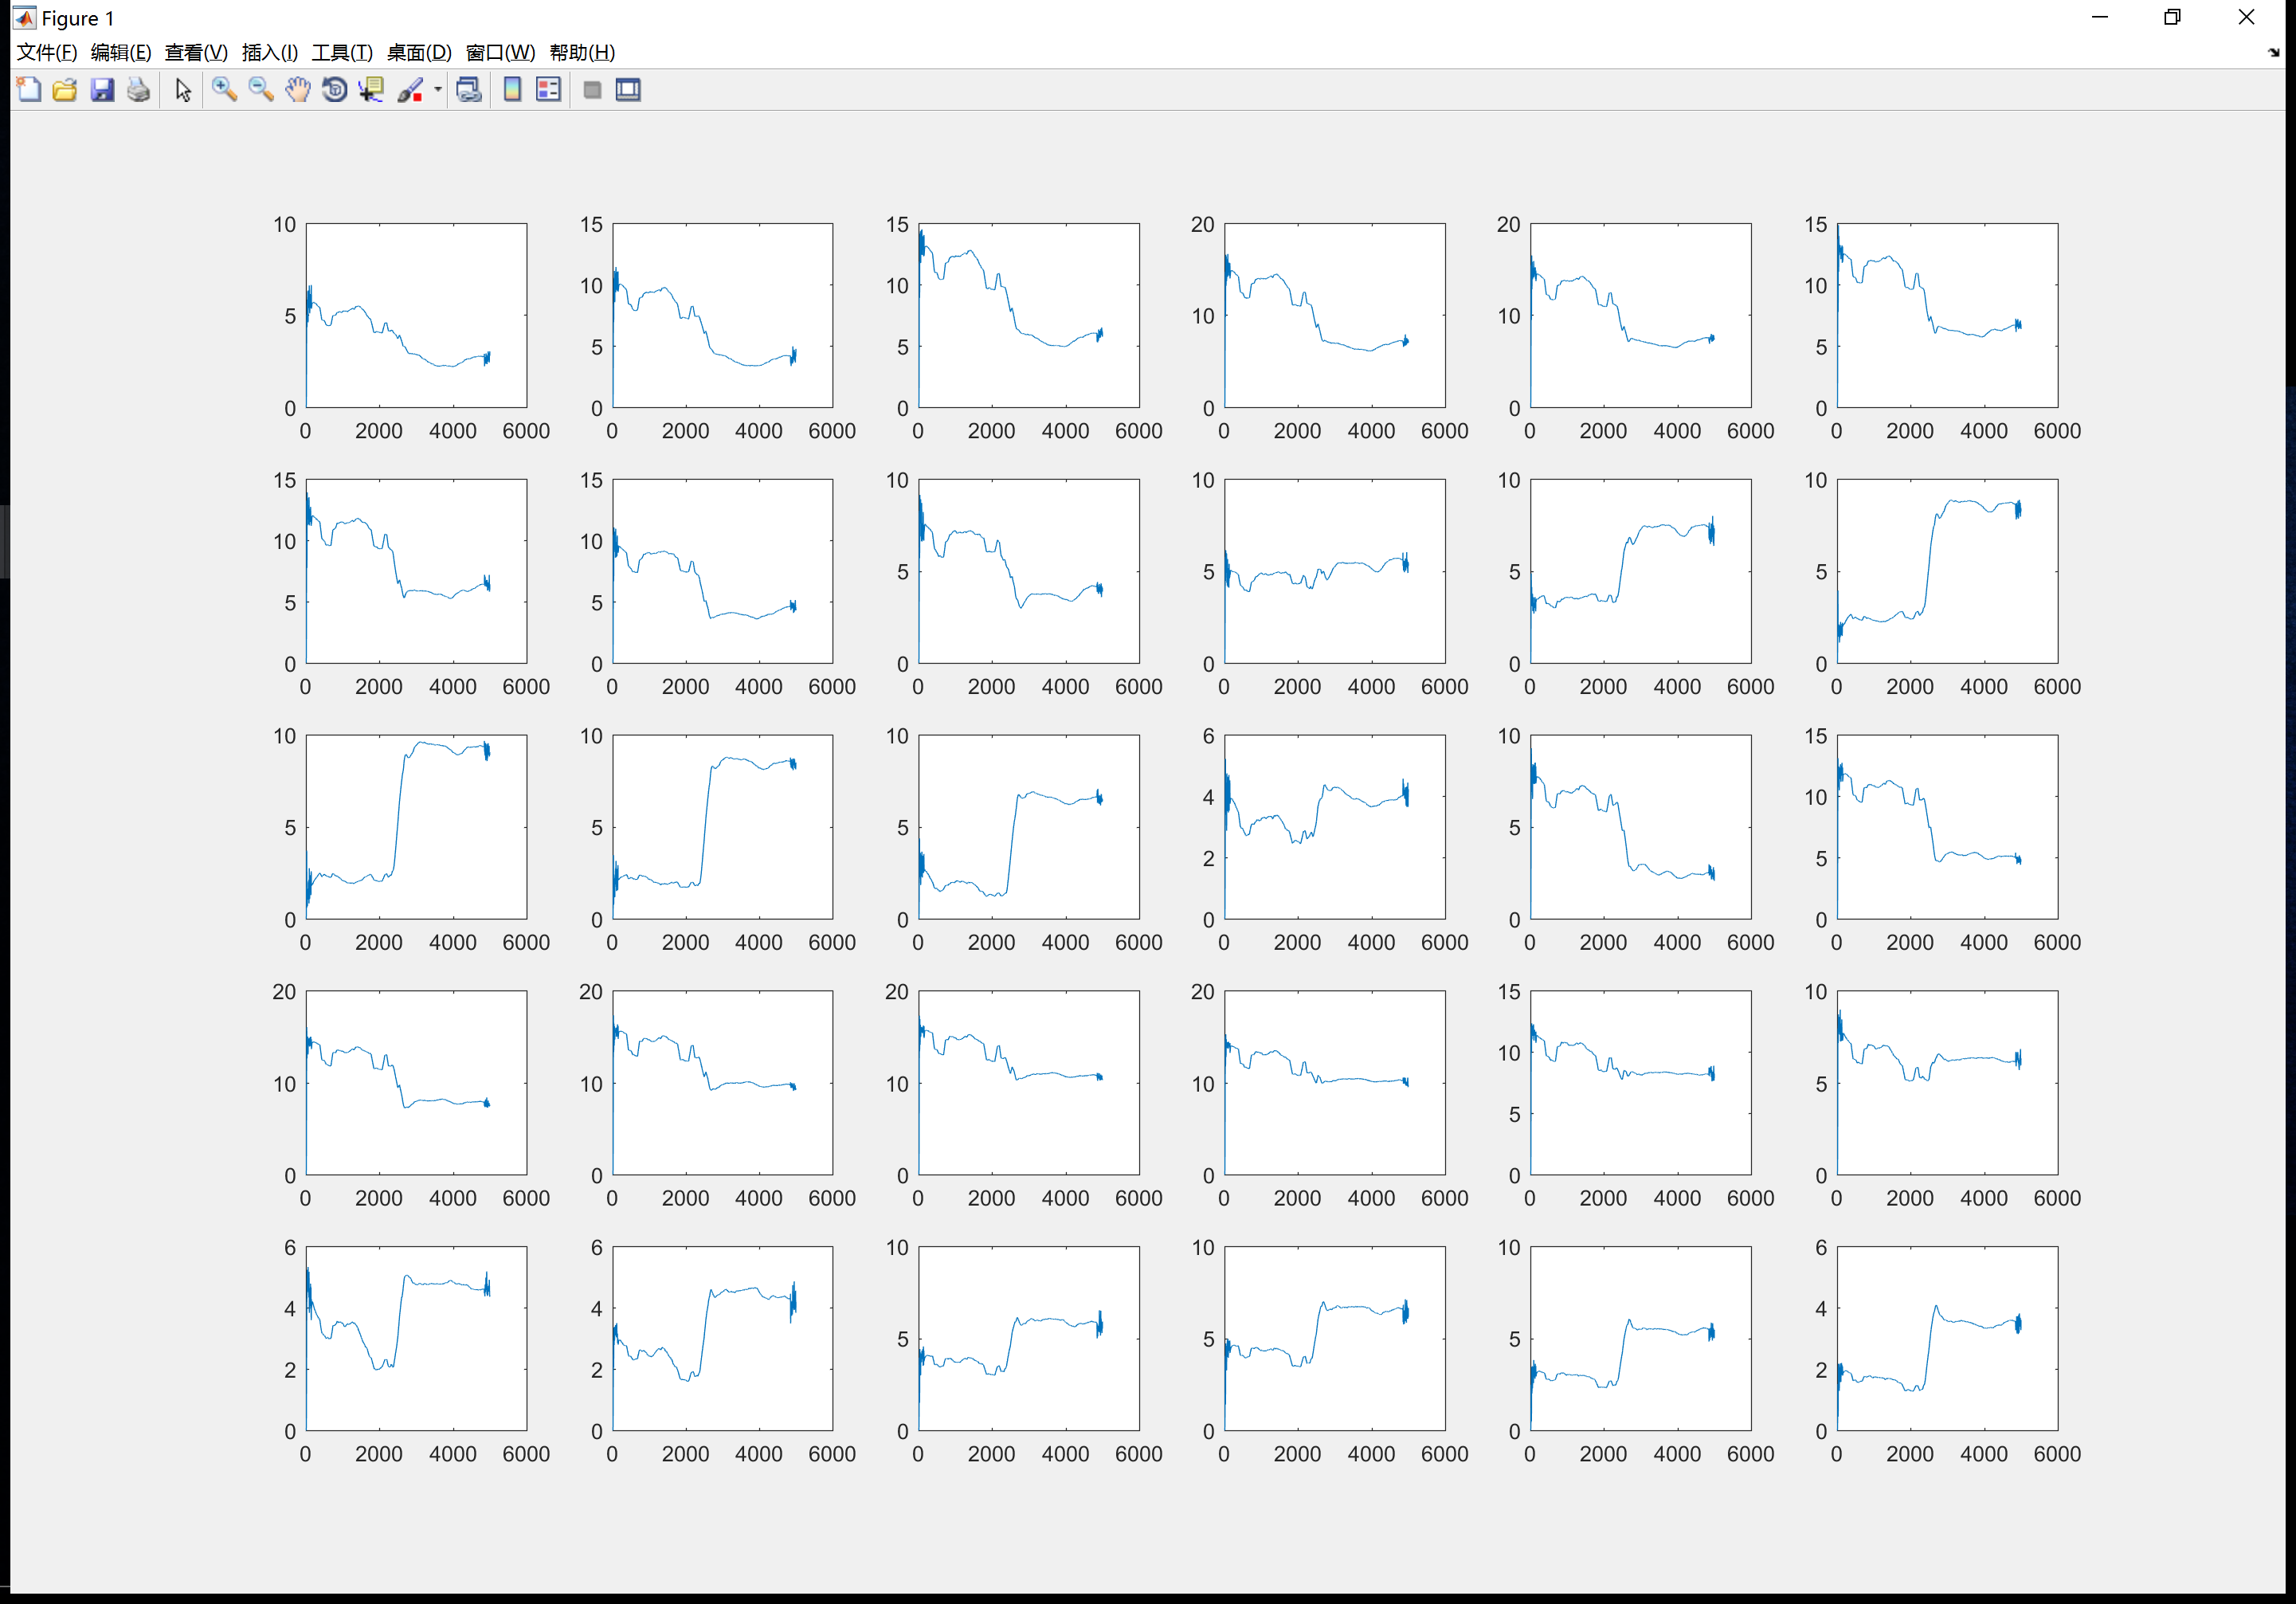
\includegraphics[width=3in]{PUSH1.png}
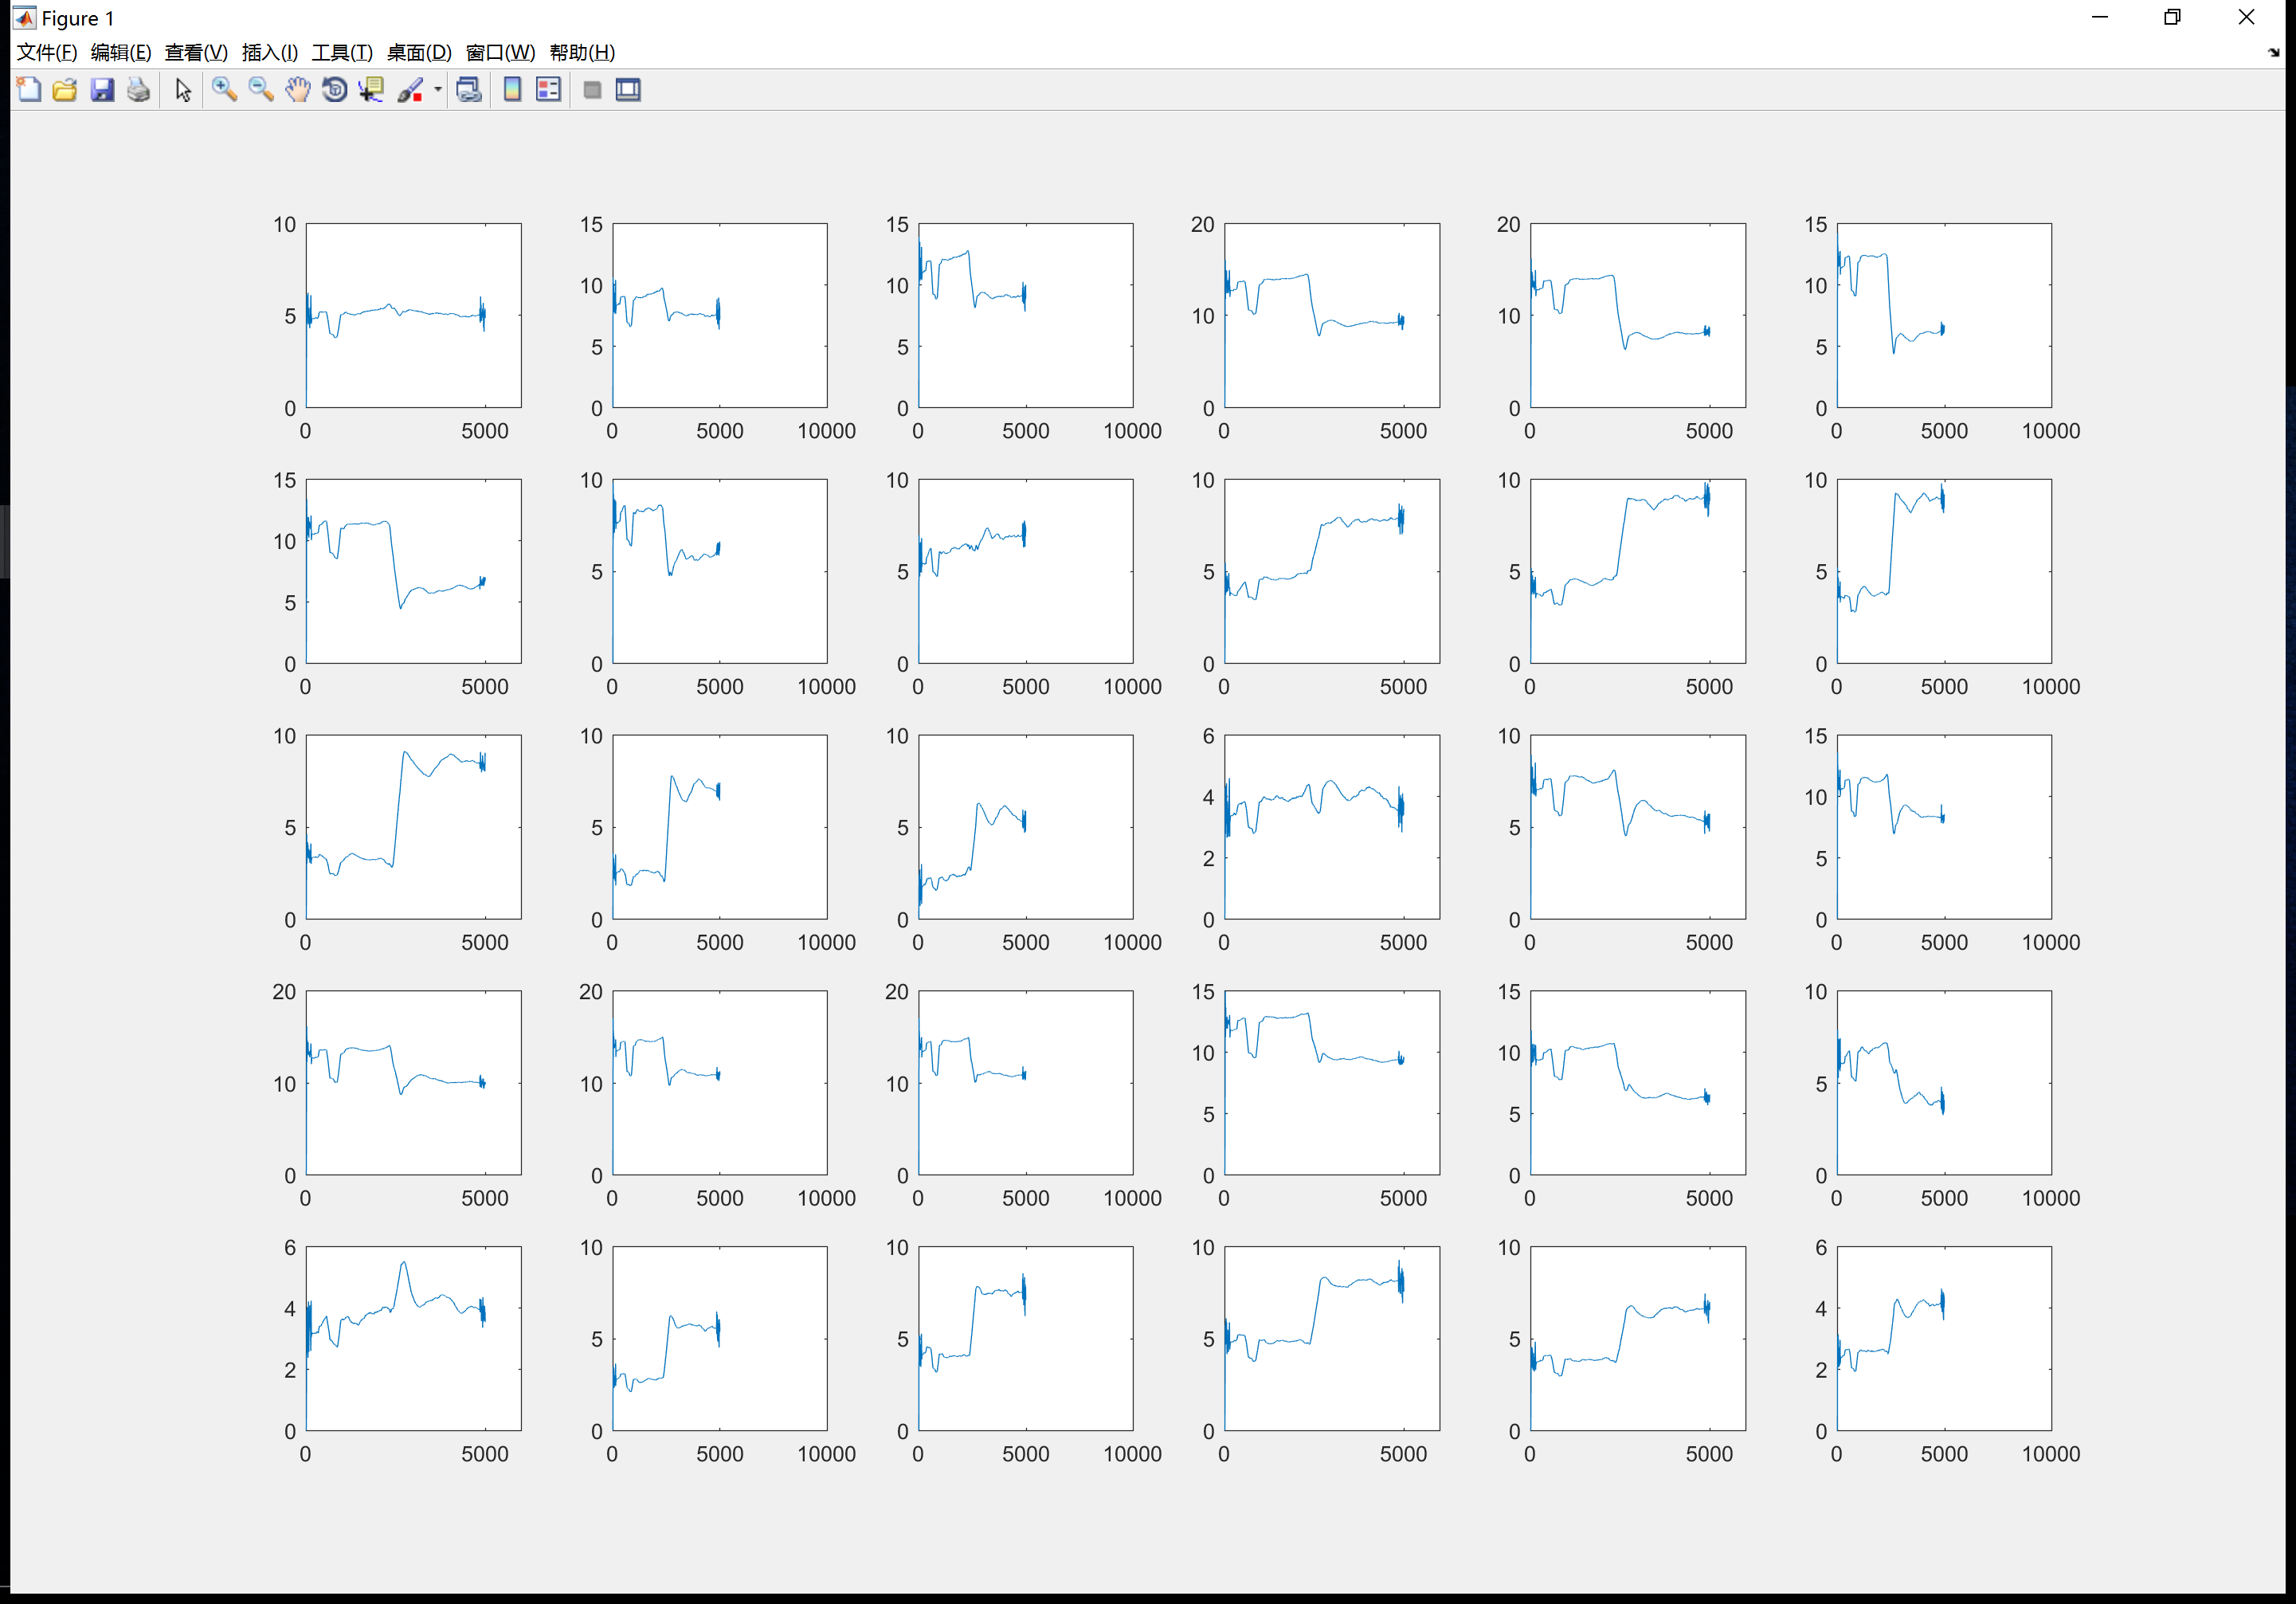
\includegraphics[width=3in]{PUSH2.png}
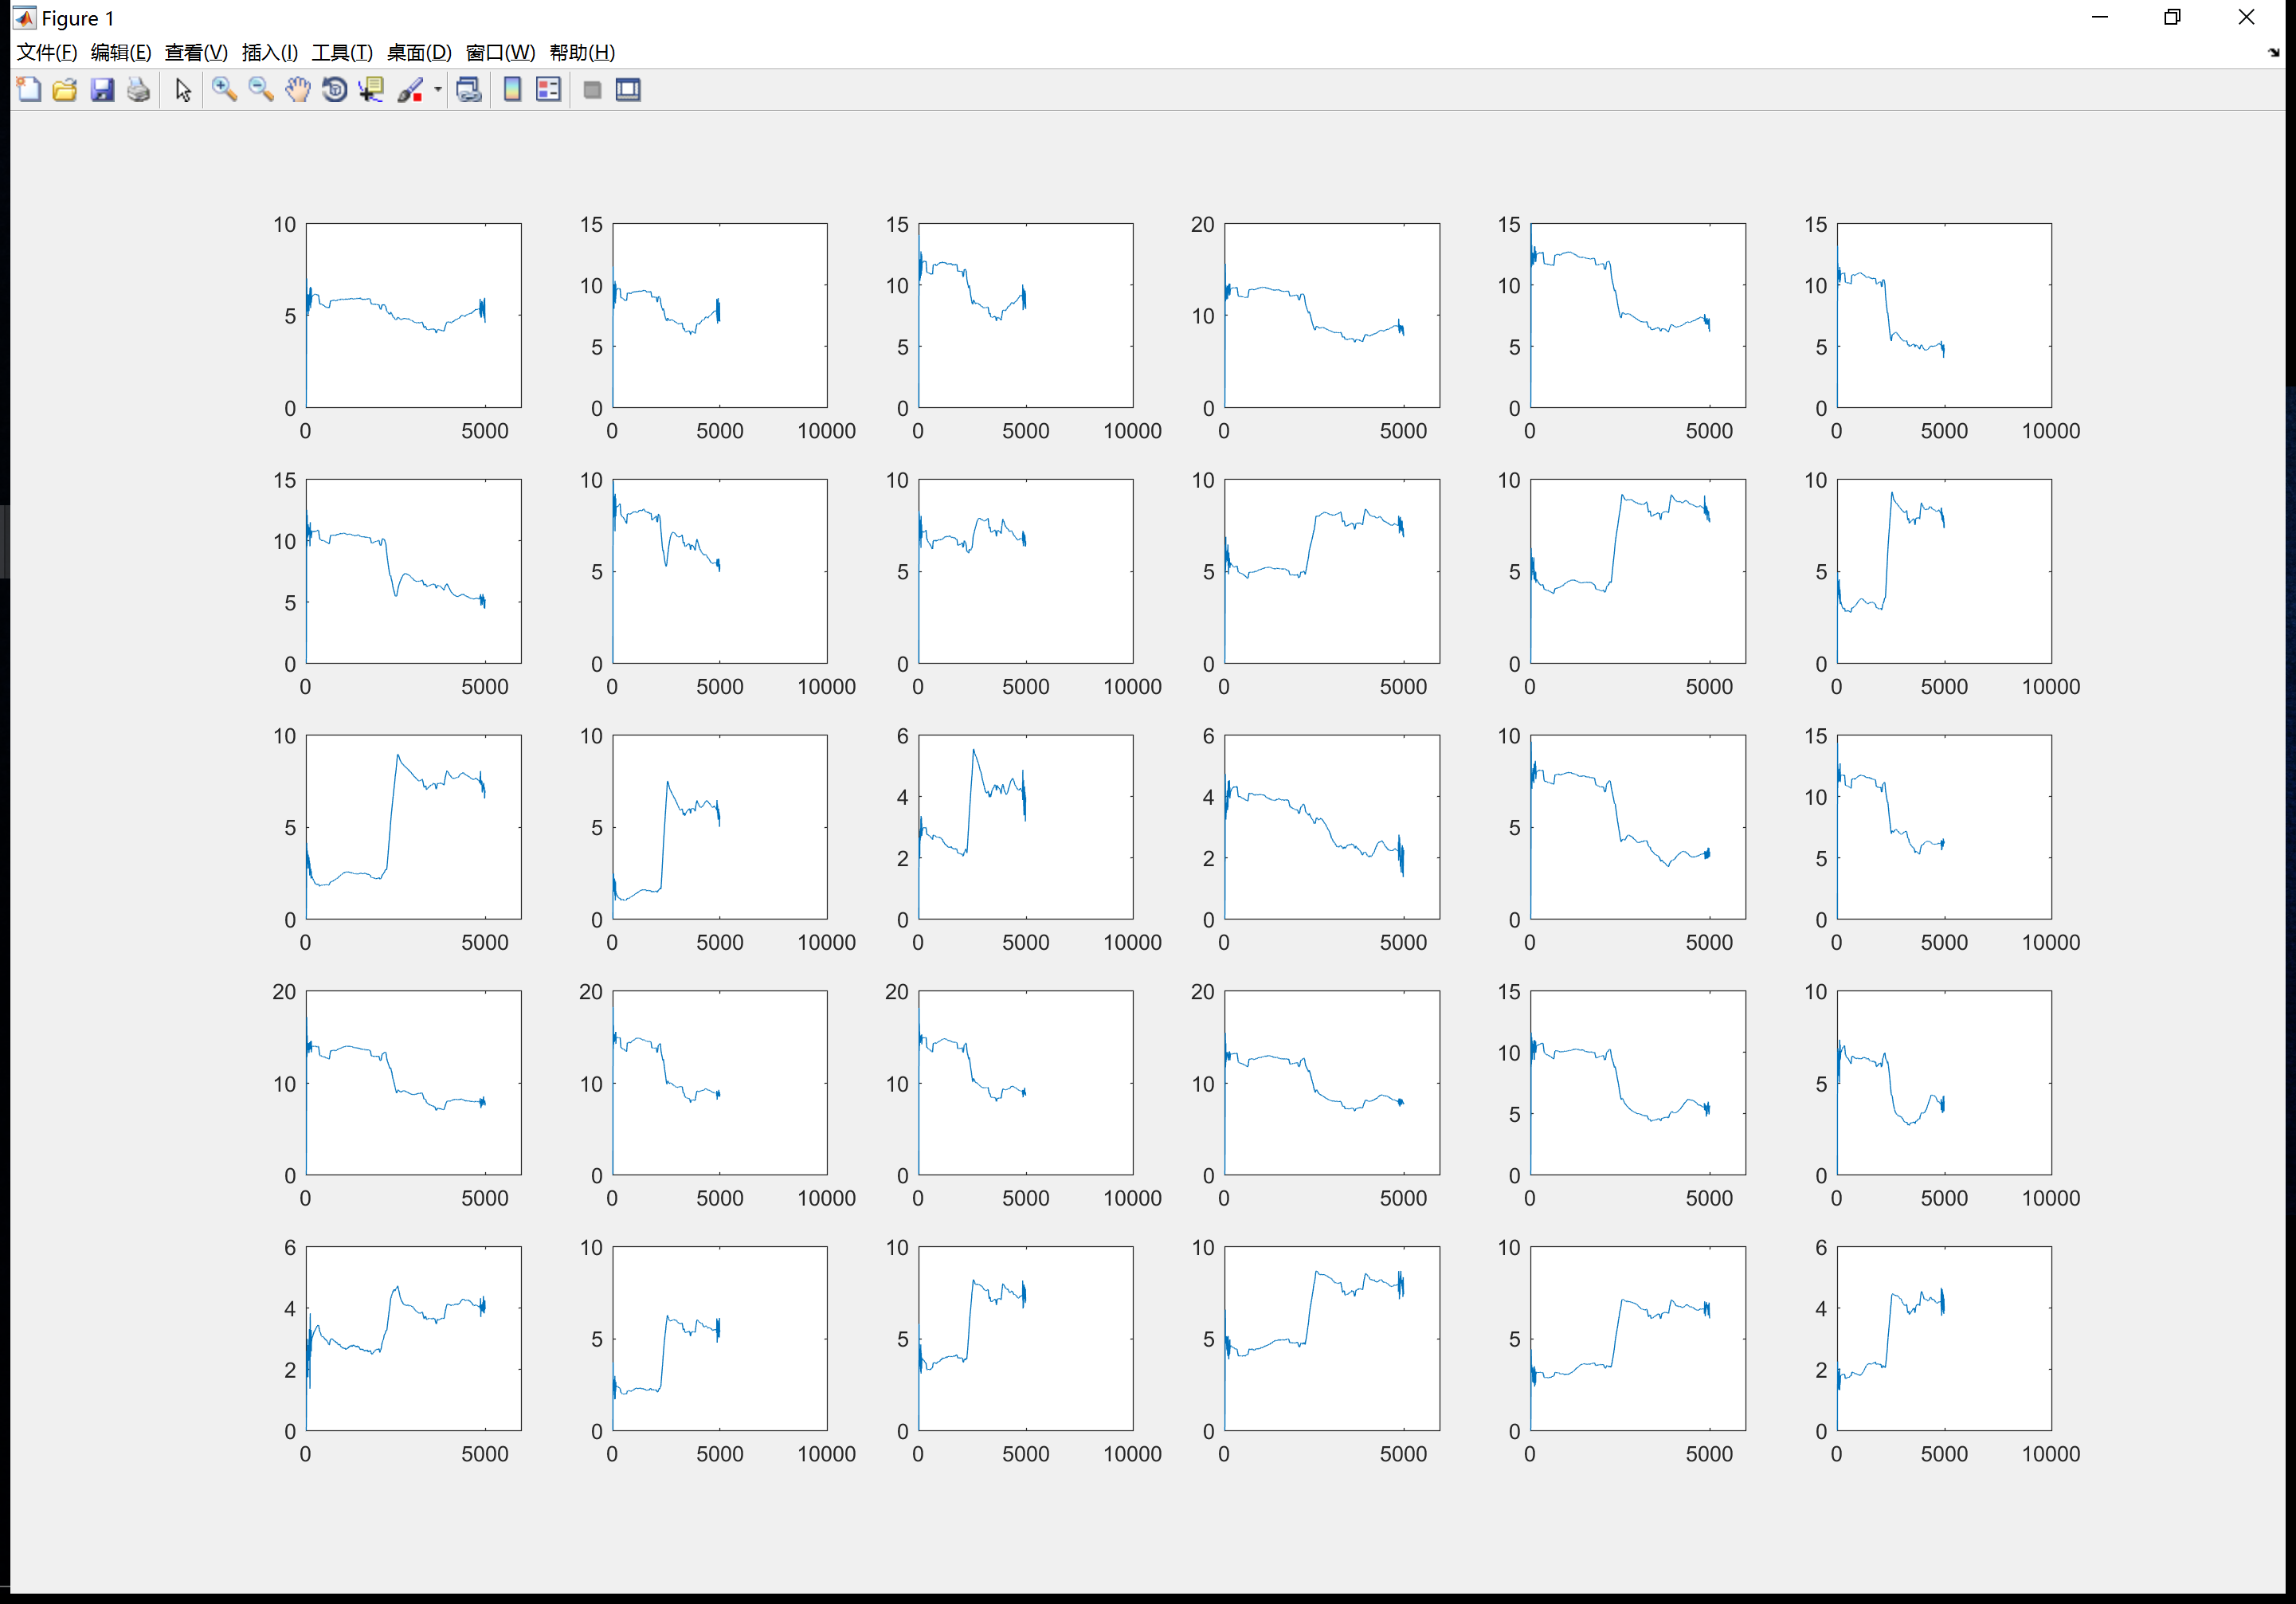
\includegraphics[width=3in]{PUSH3.png}
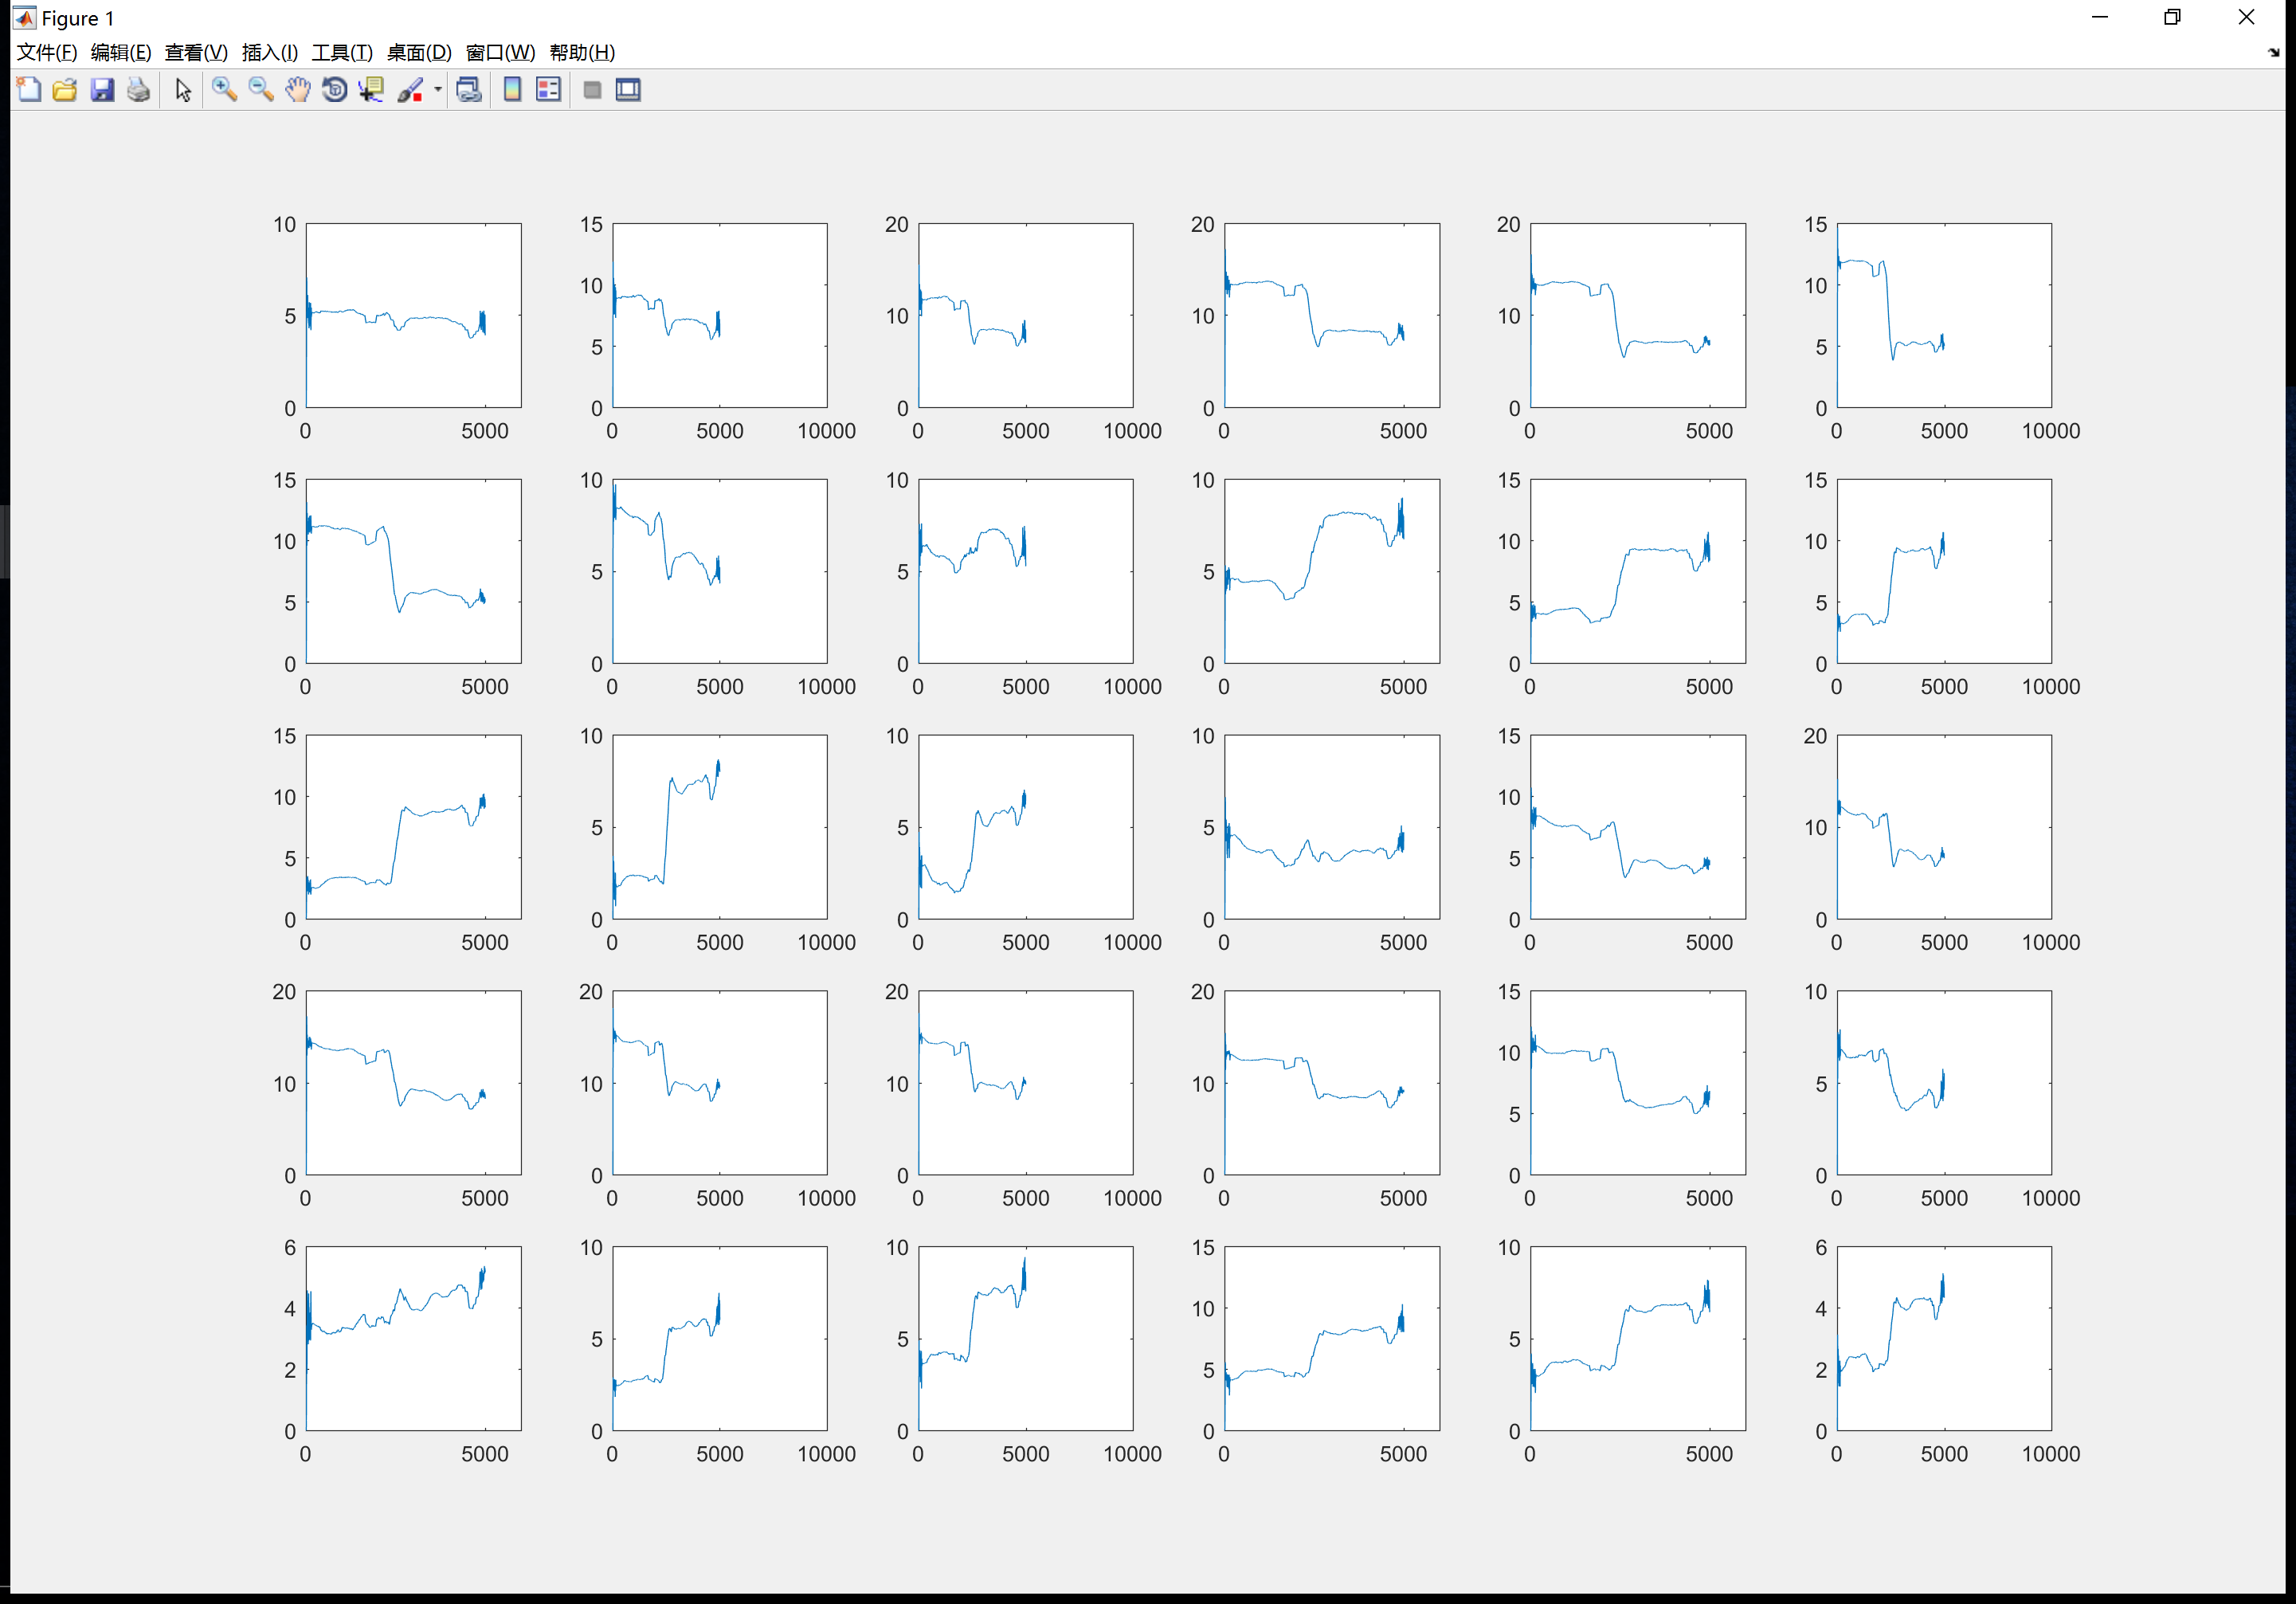
\includegraphics[width=3in]{PUSH4.png}
\caption{Signal of PUSH}
\end{figure}
The above 4 figures come from 4 independent identical gestures `PUSH'. Clearly, we can see that these signals share a very high similarity in corresponding channels.
\subsection{Model Training}


\section{Evaluation} \label{section-evaluation}


\section{discussion} \label{section-discussion}

In this section, we discuss what we learned from this project, in which division of work and future work are also covered.

\subsection{What we learned}
@SZF
\subsection{Division of Work}
Yuning Mao is the team leader. He took great efforts to the research and survey of papers in which CSI is used. He installed the hardware and set up the environment of CSI tool in Ubuntu 12.04. He tried things first and assigned tasks to the team members after having a basic understanding. He modified the program in CSI tool which was originally used to save CSI into binary file into a program which was then used to do gesture recognition. He is also responsible for most experiments and batch files.

Yuting Jia is in charge of the model, including feature selection, model selection, model training and so on. He also rewrote the C file which was originally called within \emph{matlab} in the CSI tool so that we could leverage the CSI directly.

Zhenfeng Shi did the work of signal processing. He tried multiple methods of signal filtering and implemented them in both \emph{matlab} and \emph{python}.

\subsection{Limitations and Future Work}
Currently our system depends on the environment heavily and is sensitive to noise. Due to this fact, we have to train different parameters of model in different scenarios. We think that there are a couple of reasons accounting for that. 
First, we couldn't find a quite and stable environment for data collection. The training data are hence with great noise, which is apparently undesirable. 
Second, the samples we collected are far from enough compared to the researchers who have been working on this field for years. For instance, in \cite{ali2015keystroke}, they obtained $10 persons \times 30samples/person/classes \times 37classes = 11100$ samples. We only have around one percent of them in each experiment. After all we had to collect data after establishing the whole system, and there was only one week or so and the exams were around the corner. In addition, the devices we use are old, which may cause unexpected consequences like heavy noise.

Our system also has low response since currently we don't detect the starting point and ending point of a gesture due to the limitation of time. A possible solution is to use preamble as in \cite{pu2013whole}. That is, to let user do a certain gesture first whenever he wants to use the system. The advantages of this method are that it's relatively simple to implement and can also serve as a password of a specific user. The disadvantages, however, are also apparent: it's obviously not user-friendly.

Future work directions are as follows. There are a mass of things we can(should) do if we have more time. First, We need to collect more training data in a relatively stable environment so that the quality is high enough. Second, we should try more advanced filtering methods via which we can hopefully eliminate random noise. Third, we should recognize the starting point and ending point of gestures. Furthermore, we can try different models and different applications such as keystroke recognition and voice recognition, which are more challenging and exciting in the meantime!

\section{conclusion} \label{section-conclusion}
In this project, we did various experiments by leveraging channel state information (CSI) of WiFi signals using \emph{CSI Tool} and Intel 5300 NIC.
We install the Intel 5300 NIC into a Lenovo R400 laptop and use external antennas to receive signals better.
We process the CSI and use SVM to train models to classify four different gestures and acquire an average accuracy of ??\%.
In addition, we use CSI to localize tables in the lab and achieve an average accuracy of ??\%.
It's true that there are still flaws and limits in our system. But We indeed started from scratch without instructions from the experienced and did plenty of experiments. It's pretty cool to try and learn new stuff as awesome as this from the very beginning. We learned a lot from it.

\section*{Acknowledgment}
We want to say thanks to Zhenyu Song, who let us know the CSI Tool and provide us with Intel 5300 NIC and laptop Lenovo R400. We thank Prof.Jia for the WiFi router and instruction. We also thank TA.Zhang's help.

\bibliographystyle{IEEEtran}
\bibliography{IEEEabrv,repo}
% that's all folks
\end{document}


